\documentclass[12pt,oneside,a4paper]{article}
\usepackage{graphicx} 
\usepackage{times}
\usepackage{extarrows}
\usepackage[table,xcdraw]{xcolor}

\setlength{\parindent}{0pt}
\begin{document} % 开始正文
\title{\huge SANE Dashboard}
\author{Ye Song}
\maketitle
\thispagestyle{empty}

\section{\LARGE Motivation}
SANE(Server Access Network Entity) is a set of crowdsourcing proxies, which plays a important role and act as intermediaries between between crowdsourcing clients and crowdfunding servers. The crowdsourcing clients are not allowed to communicate with crowdsourcing servers directly. Every request must be forwarded by SANE. The Architecture of SANE is based on DHT(Distributed Hash Table). This means, each node of SANE is responsible for a part of data storage and routing.  The whole architecture is completely decentralized.\\\\
Kademlia is a typical implementation of DHT designed by Petar Maymounkov and David Mazières in 2002. Each node within the DHT is identified by a unique node which is generated without taking real geographical position into account.  Within SANE the logical distance between nodes is represented by exclusive or (XOR) of the two node IDs. Due to the geographical independence of traditional Kademlia protocol, the clients of crowdsourcing may be far away from the SANE service node geographically. This will always lead to intolerable network latency. Given the above fact, the author of SANE has extended the traditional Kademlia protocol by prefixing existing 160 bits ID of node with 3 bits continent code and 10 bits country code. On the one hand, geographical position has been considered by computing the ID of node. On the other hand, the existing protocol of Kademlia has been respected seamlessly.\\\\
Our project, SANE Dashboard is designed for visual management of single SANE node. The project is found on existing project SANE and provides features of checking current node status, looking up user or device information, displaying statistical data, geographical information and submissions of crowdsourcing clients. In addition, the system is also capable of presenting the last geographical position of users and hierarchy of neighbors within the K-Buckets.

\section{\LARGE Related Work}

\subsection{\large Related Work}
\subsubsection{MapBiquitous}
The system MapBiquitous was designed by Thomas Springer, Tenshi Hara, Gerd Bombach and Sina Grunau. MapBiquitous aims to provide integrated system for indoor/outdoor location-based services. It plays the role of middleware that  provides uniform interface for applications built on different positioning technologies to bridge the heterogeneity between these technologies. It uses open standards for modeling building data with geometric and semantic information. MapBiquitous is based on C/S architecture.\\\\ 
The fat client is responsible for: \\
1 Storage of building data based on hybrid location model(both geometric and semantic location information)\\ 
2 Render gets necessary building data from loader module and enables the visualization of the data, the building data is represented on top of map layer.\\
3 Locator is built on top of a set of different positioning technologies. A common high level interface is provided on top of these technologies to bridge the heterogeneity between them.\\
4 Loader could be triggered by render module to retrieve building data from the building server that is responsible for the current building. The search for building servers is via directory service.\\\\
MapBiquitous Server: The building data and positioning infrastructure are stored on building servers, including building geometric information(floors, rooms, stairs, et cetera) and semantic information(room type, room number, et cetera). User is able to navigate a building using a MapBiquitous client that connects to a building server which maintains building information. Weather some areas of the building is public or not, depends on owner. This means, private information could be well protected.\\\\
Directory Service: Theses building servers are architecturally decentralized and could be found via Directory Service. Directory service is based on WGS84 coordinates and has been implemented using J2EE specifications(Tomcat, JSP) and MySQL. Directory Service supports search for building servers by name, longitude and latitude box. Open source project MapServer is applied for building data provisioning.\\
\begin{figure}[htb]
\centering
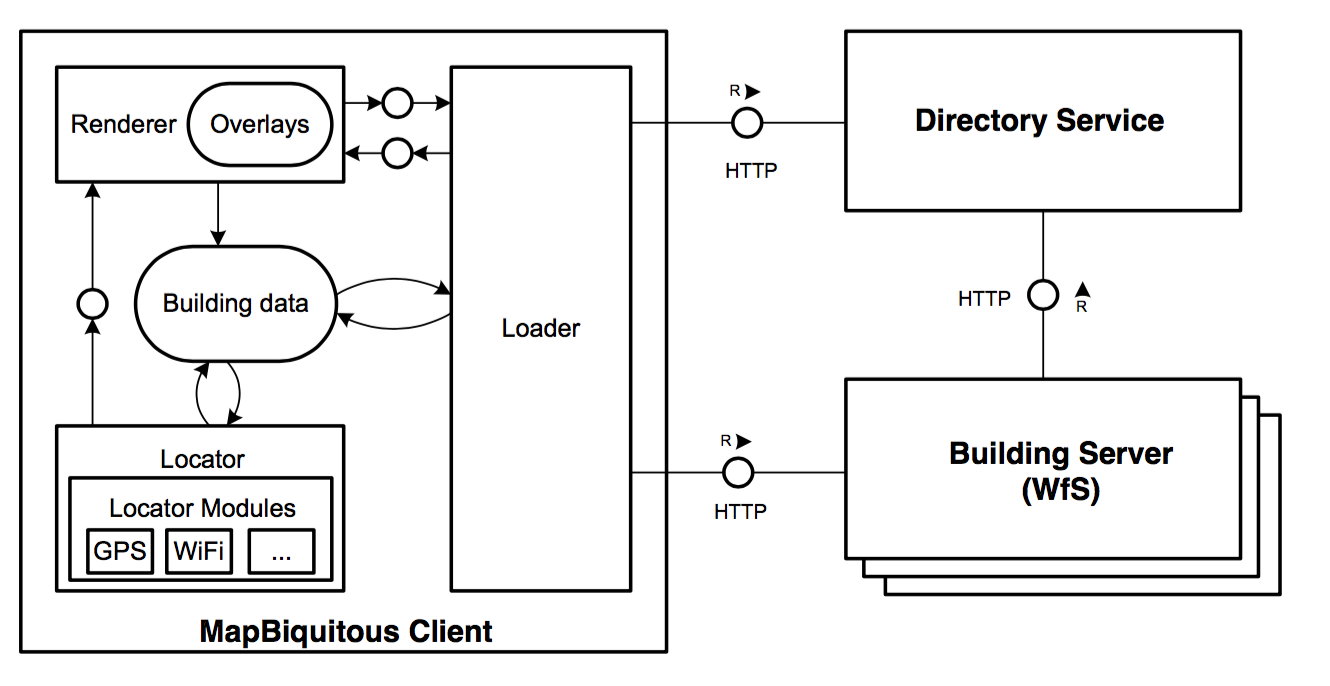
\includegraphics[width=250px, height=150px]{mapbiquitous.png}
\caption{Architecture of MapBiquitous}
\label{picture-label0}
\end{figure}
\subsubsection{SANE}
SANE(Server Access Network Entity) has been put forward and designed by Tenshi Hara in his paper ``Decentralised Approach for a Reusable Crowdsourcing Platform Utilising Standard Web Servers''. SANE plays the role of middleware platform that simplifies development of crowdsourcing applications. SANE is architecturally based on Distributed Hash Table that is a typical decentralized structure. Each node within a DHT is responsible for partial data storage and partial routing. Figure 2 shows the mechanism of DHT of SANE. SANE 1 is responsible for area[0-3], as well as area[c-7]. SANE is responsible for area[4-7], as well as area[0-b]. SANE 3 is responsible for area[8-b], as well as area[0-f]. SANE 4 is responsible for area[c-f], as well as area[8-3]. The hashed userid of client begins with character `b', the node of SANE that is responsible for area `b' is SANE 3 [8-b].Its upper neighbor SANE 2 and lower neighbor SANE 4 act as backups.\\\\
\begin{figure}[htb]
\centering
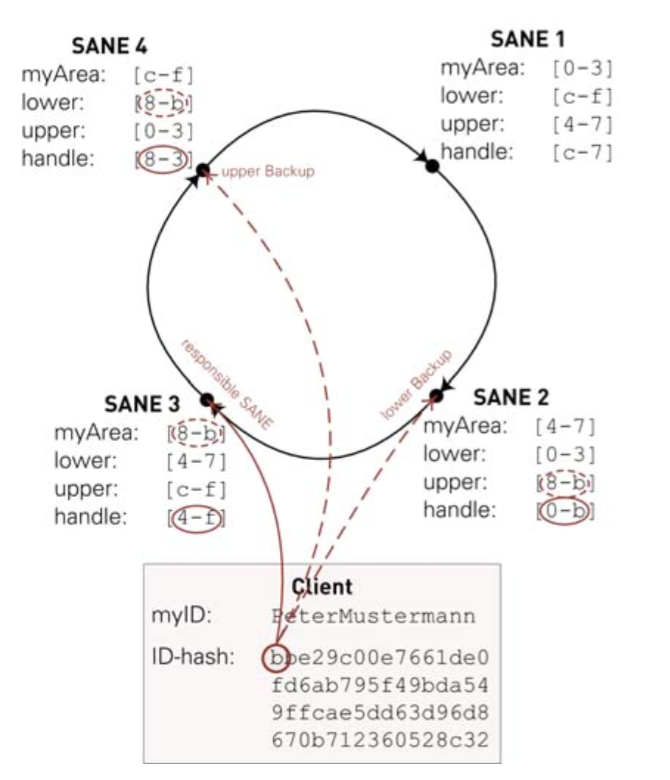
\includegraphics[width=150px, height=150px]{sanedht.png}
\caption{DHT of SANE}
\label{picture-label01}
\end{figure}
There is no central node within a DHT, this property eliminates bottleneck at central node in a traditional centralized network. DHT is an efficient approach to organize huge numbers of nodes and construct a decentralized network. A node could be easily added to or removed from a DHT network. This means, SANE is well scalable to deal with vast numbers of clients. Given fault tolerance, each node is responsible for backups of its neighbors via storage of partial extra data. SANE enables user management, client management, server management, DHT maintainer and security. SANE ensures that all internal communication between modules are signed and encrypted. SANE also ensures that all write-access to crowdfunding servers must be re-signed and re-encrypted to keep the submitted data traceable. SANE store all additional information related to the submissions, the submissions are stored on crowdfunding servers. SANE project has been implemented using standard technologies LAMP(Linux, Apache, MySQL, PHP). MapBiquitous's Android client could communicate with SANE proxy by simply adding a SANE library, this means, SANE acts as a mediator between MapBiquitous clients and MapBiquitous servers.
\begin{figure}[htb]
\centering
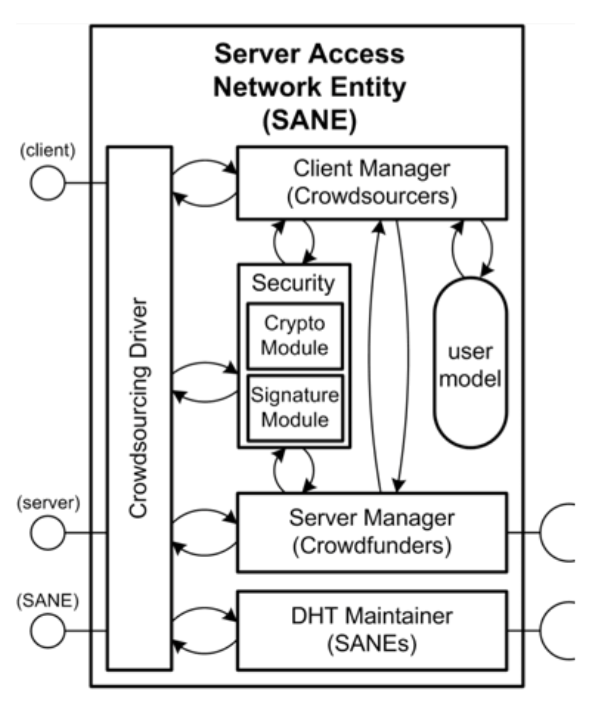
\includegraphics[width=250px, height=150px]{sane.png}
\caption{Architecture of SANE}
\label{picture-label00}
\end{figure}

\subsubsection{Location based DHT}
Kademlia(Kad) is a typical structured P2P overlay network. It aims to solve information storage and retrieval in distributed environment. In Kademlia network, all information is stored in the form of entries within a hash table. These entries are discretely stored on each node, thereby constituting a huge distributed hash table. The huge distributed table could be considered as a large dictionary. As long as we know the key of the information, we will be able to query its corresponding value information through the Kademlia protocol regardless of the physical position of the node. Each node within a Kad network has a unique ID that is a 160 bits hashed value. It is considered almost impossible that two nodes have the same ID. In the Kad network , the distance between two nodes don't depend on the their physical distance. In fact, the distance is calculated by the XOR operation. We assume that there are two nodes, a and b, the distance d = a XOR b, the larger the value of d, the larger the distance between a and b. The distance calculated by XOR is only a logical distance regardless of physical position.\\\\
In Kad network, each node maintains 160 lists, each of which is called K-Bucket. In list i, neighboring nodes that are 2\^{}i $\sim$ 2\^{}(i+1) away from current node are stored in the form of (Node ID,IP,UDP port) tuple. Default value of K is 20. \\
The update of K-Buckets follows these principles:\\
1 The list is not full(number of nodes less than K), if the queried node is not in the list, the node will be added to the tail of list. If the node is already in the list, then the node will be moved to the tail of list.\\
2 The list is already full, and the queried node is not in the list. If the head node is still active, the new node will be thrown, the head node will be moved to tail, else the head node will be removed and the new node will be added to tail of list.
\begin{figure}[htb]
\centering
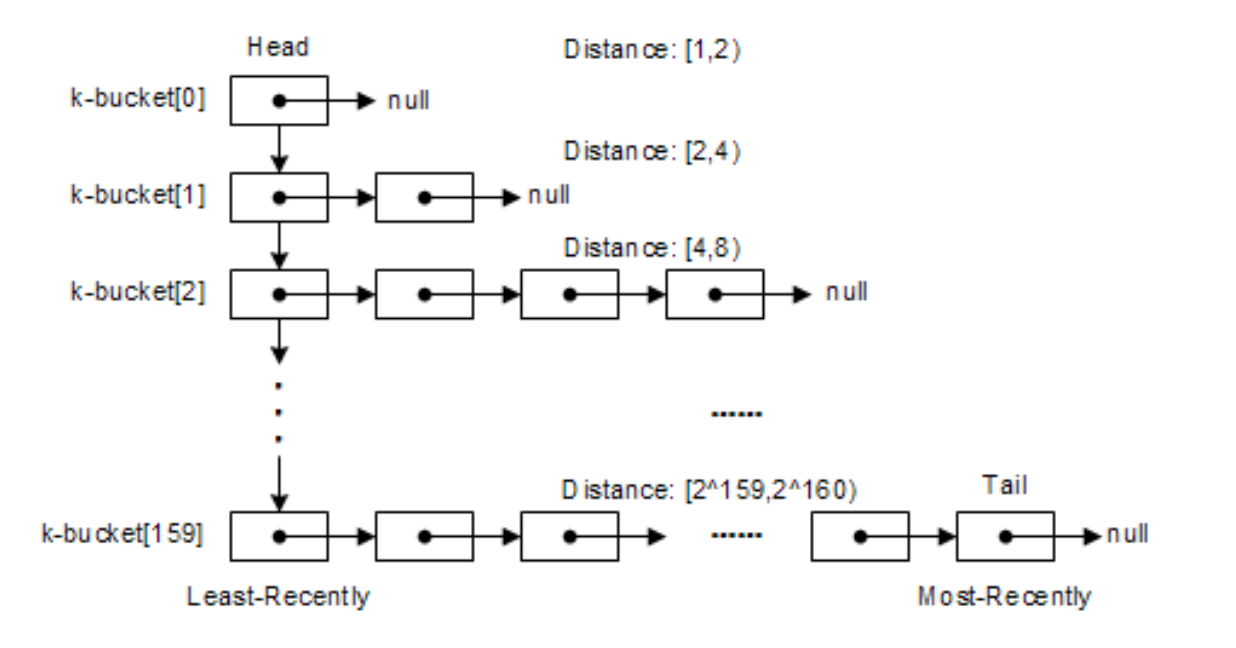
\includegraphics[width=250px, height=150px]{kbucket.png}
\caption{K-Buckets}
\label{picture-label001}
\end{figure}

Kademlia network doesn't take real position into consideration. The means, service node that is responsible for the current client might locate far away from the client. The will cause unnecessary network overhead and compromise user experience. For this reason, Hara proposed a solution in his paper ``Decentralised Approach for a Reusable Crowdsourcing Platform Utilising Standard Web Servers''. Basically this solution is based on DNS to retrieve nearby service node for the client. Steps of this solution are shown in the following figure:\\
\begin{figure}[htb]
\centering
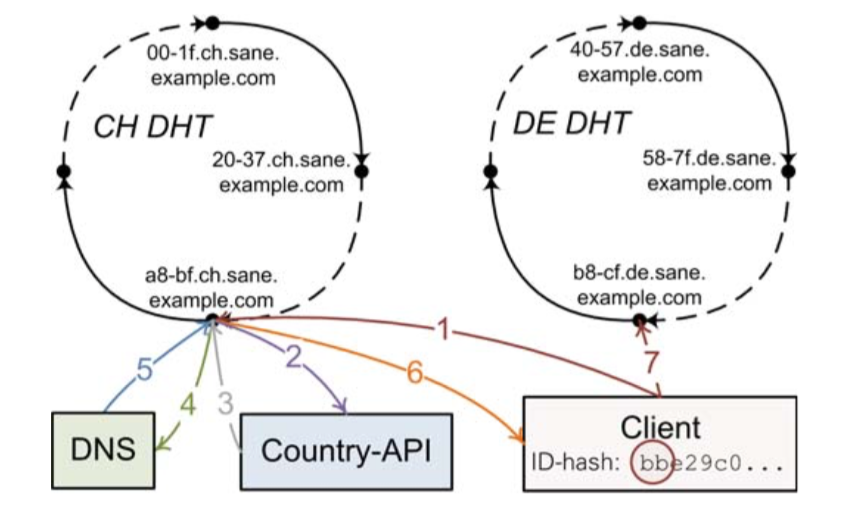
\includegraphics[width=250px, height=150px]{sanedns.png}
\caption{Solution based on DNS}
\label{picture-label002}
\end{figure}
Step 1: A client that locates in US contacts service node locating in Germany.\\
Step 2, 3: Service node determines where the client comes from via Country-API.\\
Step 4, 5: Service node gets another service node locating in US via DNS.\\
Step 6, 7: Client contacts the new service node that is responsible for its area.\\

Given the complexity due to additional DNS, Tan Dung Nguyen proposed a new solution in his paper ``Auswahl und Implementierung eines geeigneten Distributed Hash Table Verfahrens fuer die selbstaendig regionale Verteilungen beruecksichtigende Organisation einer verteilten Prokura-Kommunikation in MapBiquitous'' basically without modification of original routing algorithm. Main idea is prefixing the existing 160 bits hash code with additional positional information that doesn't affect routing algorithm. The K-Bucket of a node in normal Kademlia network without considering real position looks like the following:



\begin{table}[!h
]
\centering
\caption{K-Buckets Considering No Real Position}
\label{my-label}
\begin{tabular}{|c|c|c|c|c|c|}
\hline
\multicolumn{1}{|l|}{Node-ID} & \multicolumn{5}{c|}{K-Buckets}                                                                                                                                                      \\ \hline
0001                          & \multicolumn{1}{l|}{distance: 0} & \multicolumn{1}{l|}{distance: 1} & \multicolumn{1}{l|}{distance: 2-3} & \multicolumn{1}{l|}{distance: 4-7} & \multicolumn{1}{l|}{distance: 8-15} \\ \hline
                              & 0001                             & 0000                             & 0010                               & 0100                               & 1000                                \\ \hline
                              &                                  &                                  & 0011                               & 0111                               & 1101                                \\ \hline
\end{tabular}
\end{table}

If nodes 0001, 0000, 0010, 0111, 1000, 1101 locate in Germany, other nodes 0011, 0100 locate in US. We assume that nodes locating in Germany are prefixed with 0, nodes locating in US are prefixed with 1. Logical distance is still calculated via XOR operation. Then the K-Buckets look like the following:
\begin{table}[!h]
\centering
\caption{K-Buckets Considering Real Position}
\label{my-label2}
\begin{tabular}{|c|c|c|c|c|c|c|}
\hline
\multicolumn{1}{|l|}{Node-ID} & \multicolumn{6}{c|}{K-Buckets}                                                                                                                                                                                             \\ \hline
{\color[HTML]{333333} 00001}  & \multicolumn{1}{l|}{Dis: 0} & \multicolumn{1}{l|}{Dis: 1} & \multicolumn{1}{l|}{Dis: 2-3} & \multicolumn{1}{l|}{Dis: 4-7} & \multicolumn{1}{l|}{Dis: 8-15} & \multicolumn{1}{l|}{Dis: 16-31} \\ \hline
                              & 00001                            & 00000                            & 00010                              & \cellcolor[HTML]{FFFFC7}(0100)     & 01000                               & \cellcolor[HTML]{9AFF99}10011        \\ \hline
                              &                                  &                                  & \cellcolor[HTML]{FFFFC7}(0011)     & 00111                              & 01101                               & \cellcolor[HTML]{9AFF99}10100        \\ \hline
\end{tabular}
\end{table}
The nodes locating in US have been moved to K-Bucket 16-30, other nodes remain in original K-Buckets. The routing algorithm remains unchanged. In Dung's paper, he proposed 13 bits code to prefix 160 bits hash code. 3 bits are used to identify 5 continents. 10 bits are used for identify all countries(nowadays 241 countries in the world) according to ISO-3166 (International Organiza- tion for Standardization) without considering secondary-level region, z.B. province, city due to workload. In the following table, we show a sample of this model, we assume that Europe is coded as 010, Germany is coded as 0100010100. Our DHT module is based on this model.
\begin{table}[!h]
\centering
\caption{173 Bits Hash Code}
\label{my-label}
\begin{tabular}{|c|c|c|}
\hline
continent & conutry    & 160 bits hash code                 \\ \hline
010       & 0100010100 & 010001010001000101000100010100.... \\ \hline
\end{tabular}
\end{table}

% Organization
\subsection{\large Organization}
There are three members in our team, Guanghui Ji, Kaijun Chen and me. We met every week to share the designs for our project during analysis period. After this period, we had to meet more frequently to discuss protocol between frontend and backend, user interface design, technology selection, allocation of tasks, etc. Due to the detailed designs we could focus on implementation in the next period. \\\\
The two main tools that we applied for management and organization were Google Drive and Trello. Google Drive, formerly Google Docs, is a file storage and synchronization service created by Google. It allows users to store files in the cloud, share files, and edit documents, spreadsheets, and presentations with collaborators.
All of our analysis and designs documents, protocols, related papers, database configuration, etc. are stored in Google Drive. Given the commerciality and closed source of JIRA, we took Trello as our collaboration tool. Trello is a web-based free application that organizes our project into boards, lists, cards and gives user a visual overview of ``doing'', ``to do'' and ``done'' tasks and the persons in charge of these tasks. Trello also provides notification through Email, so that we could keep up with project progress and assign tasks conveniently.

\begin{figure}[htb]
\centering
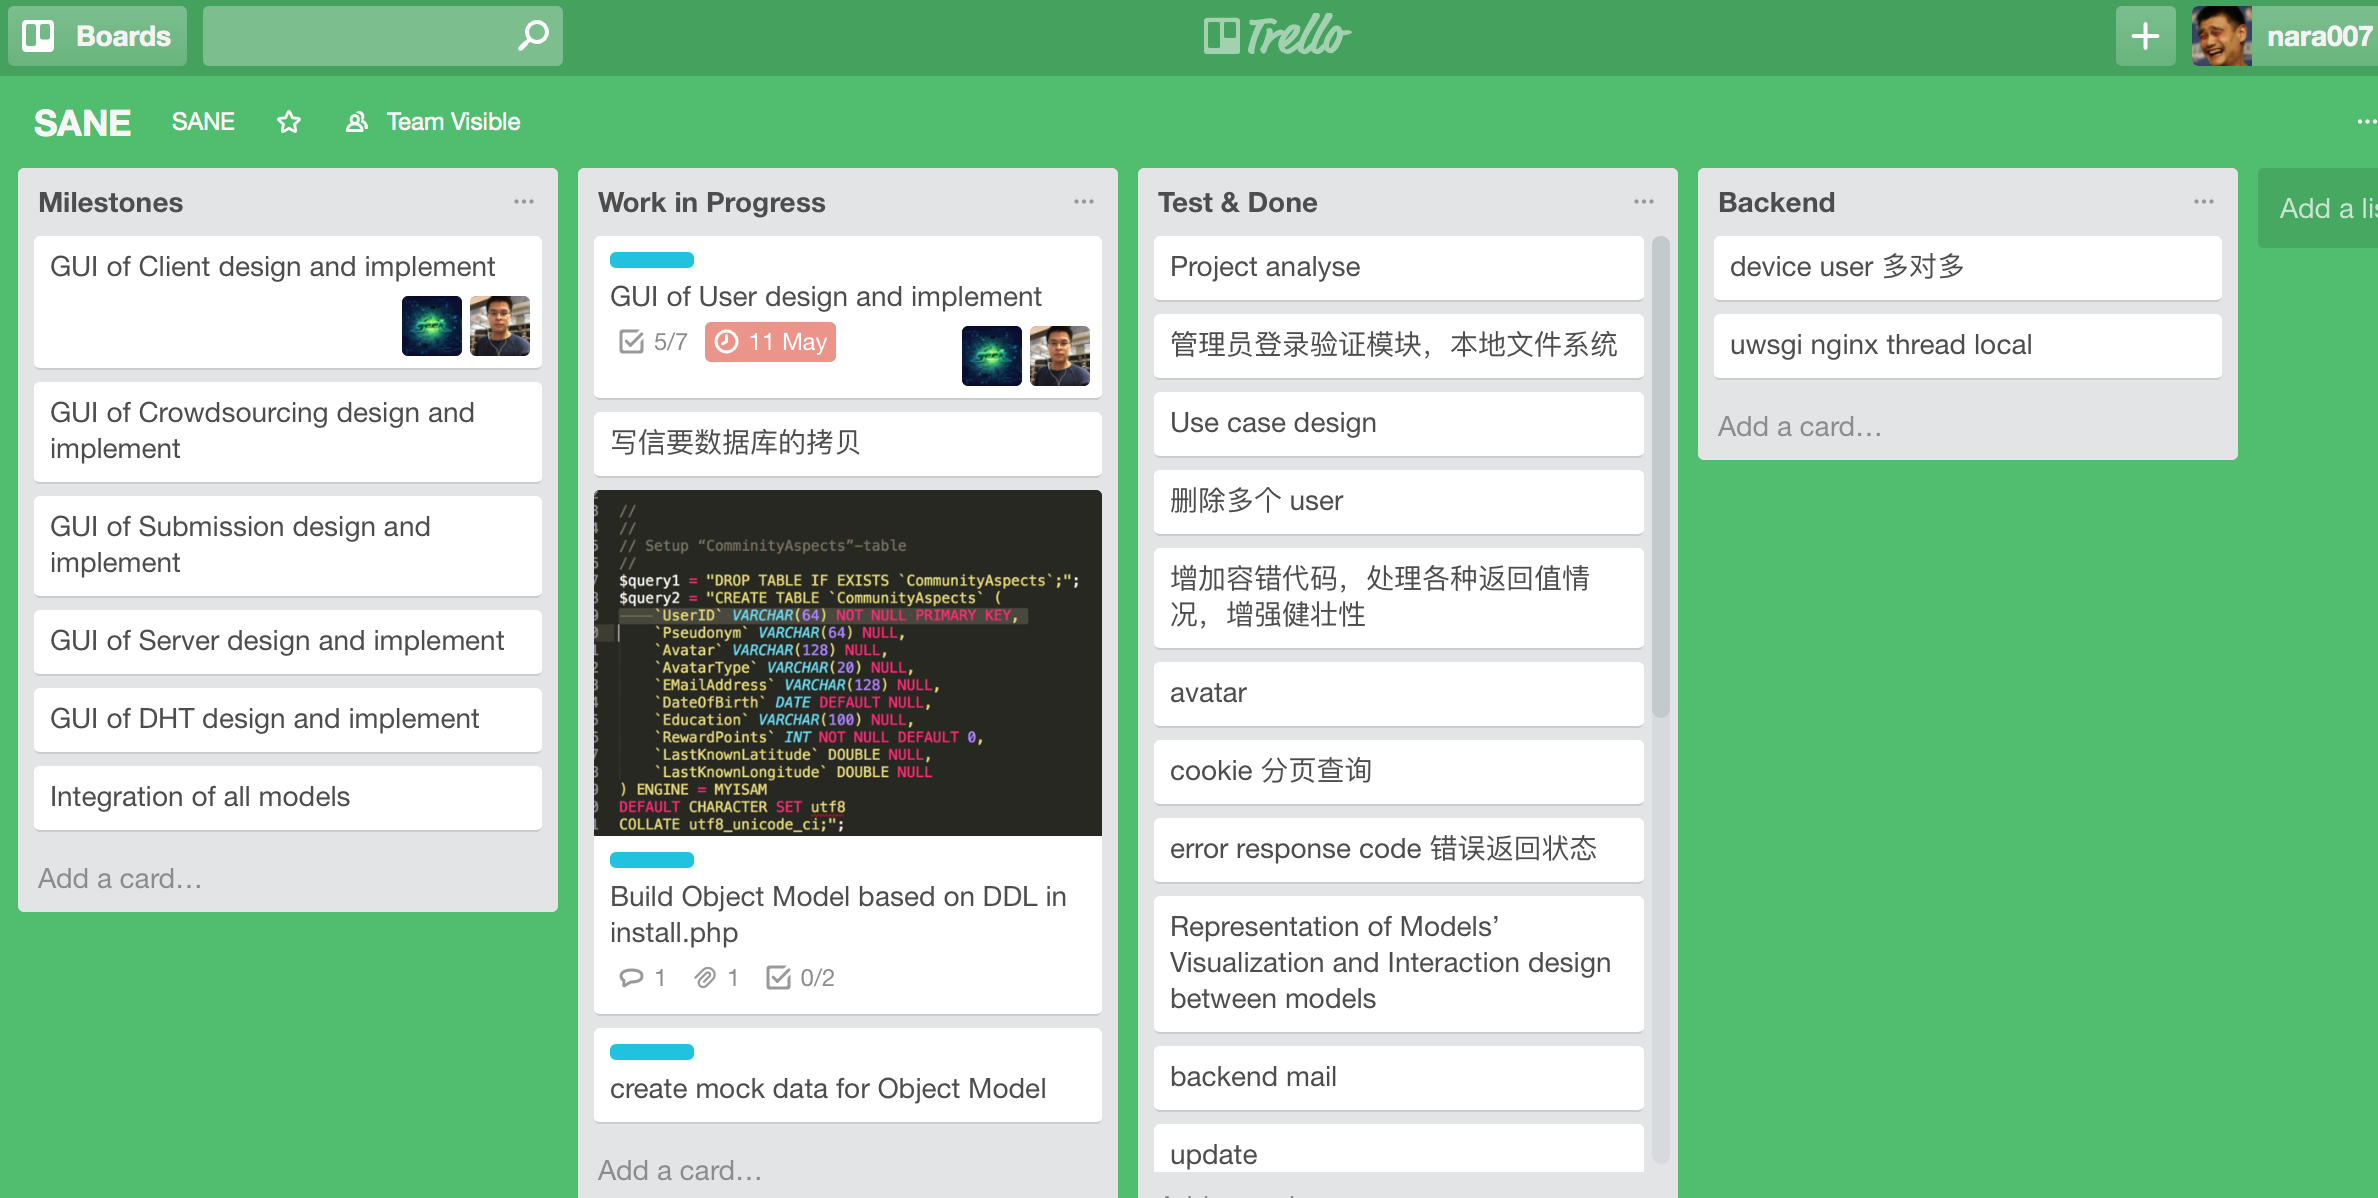
\includegraphics[width=250px, height=150px]{trello.png}
\caption{Overview of Trello}
\label{picture-label}
\end{figure}

\begin{figure}[htb]
\centering
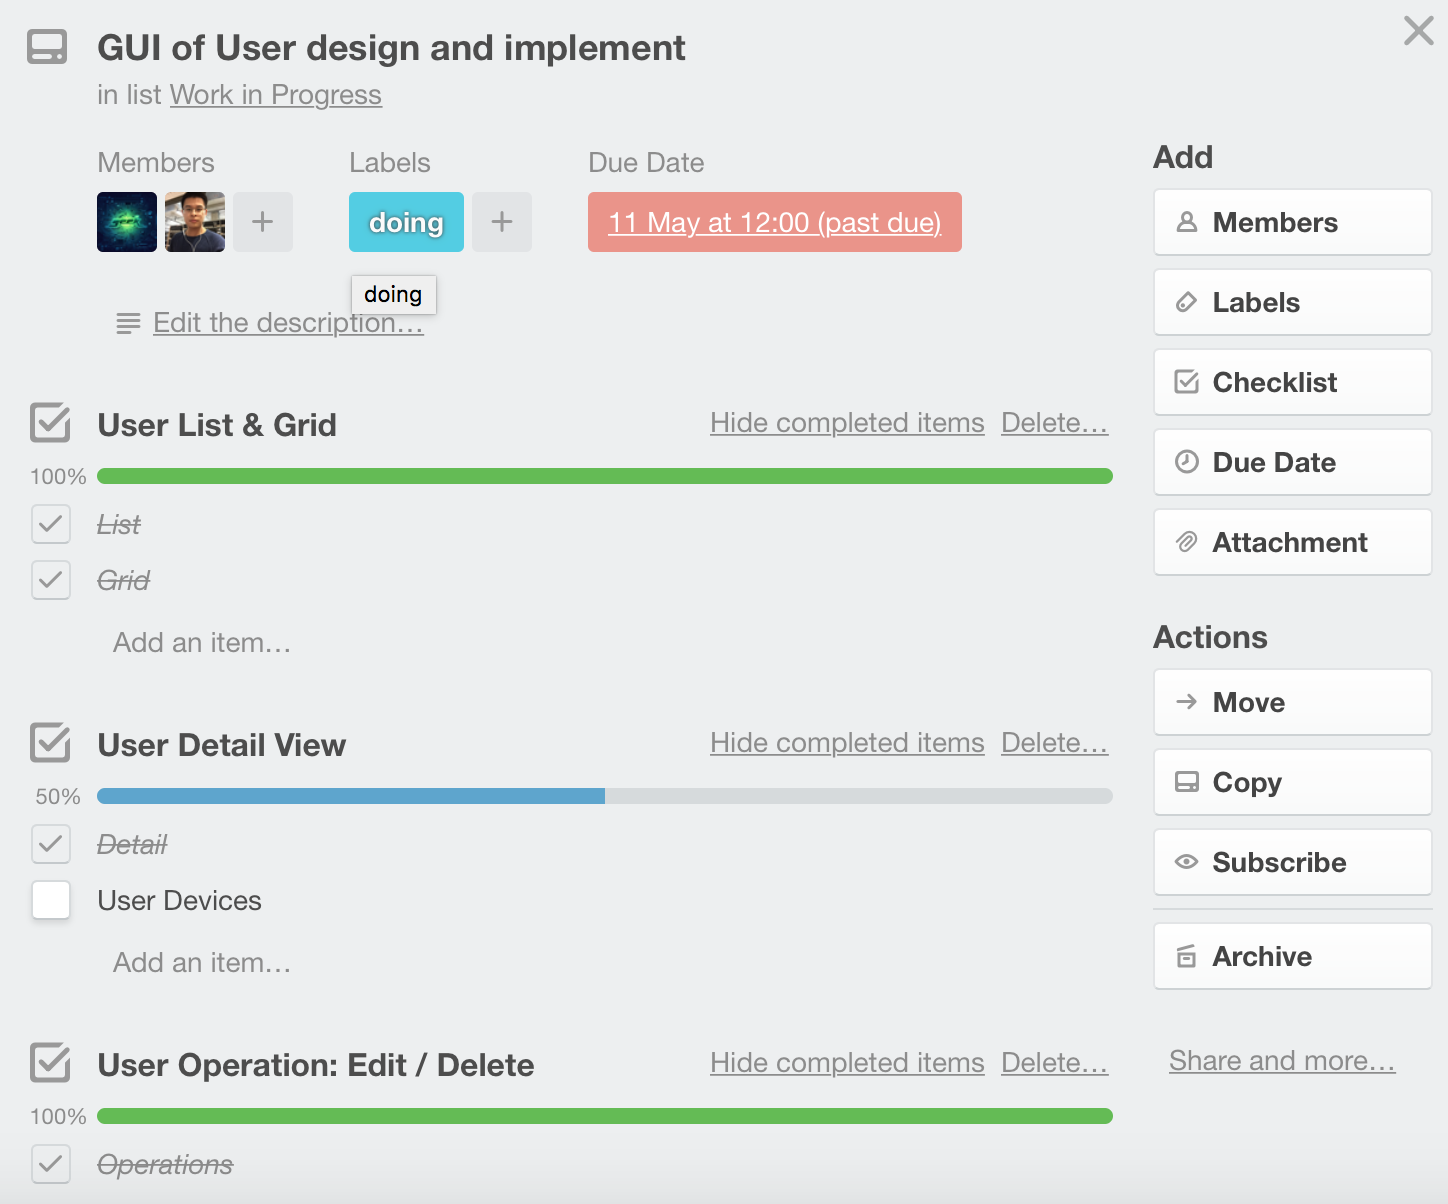
\includegraphics[width=250px, height=150px]{trello2.png}
\caption{Overview of Trello 2}
\label{picture-label2}
\end{figure}

% subsection Research of Existing Project
\subsection{\large Research of Existing Project}
The project SANE Dashboard is based upon the project SANE. Therefore we need to analyze SANE to acquire the important information, e.g. schema of tables in database, restful API provided by SANE, directory service of crowdsourcing servers, DHT neighbors within K-Buckets, etc.\\\\
Schema of tables locate in PHP module ``install.php'', e.g. table ``UserData'' and ``Devices'' as following:\\\\
\scriptsize{\textbf{\emph{CREATE TABLE UserData (UserID VARCHAR(64) NOT NULL PRIMARY KEY, Username VARCHAR(64) NOT NULL, Password VARCHAR(64) NULL, PublicKey TEXT NULL, RegistrationDate DATETIME NOT NULL ) ENGINE=MYISAM DEFAULT CHARACTER SET utf8}}}\\\\
\textbf{\emph{CREATE TABLE Devices (DeviceID VARCHAR(64) NOT NULL PRIMARY KEY, UserID VARCHAR(64) NOT NULL, DeviceSpecs BLOB NULL, RegistrationDate DATETIME NOT NULL, ModificationDate DATETIME NOT NULL, FOREIGN KEY (UserID) REFERENCES UserData(UserID) ) ENGINE=MYISAM DEFAULT CHARACTER SET utf8}}\\\\
\normalsize{Directory Service can be found under ``libs/Crowdfunder.php'':}\\\\
\scriptsize{\textbf{\emph{\$\_CONFIG[`DS']=``carlos.inf.tu-dresden.de''\\
\$\_CONFIG[`DSport']=``80''\\
\$\_CONFIG[`DSpath']=``/DS/''\\
\$\_CONFIG[`DSssl']=false}}}\\\\
\normalsize{RESTful APIs of SANE are available at http://sane.hawk310.startdedicated.de. We can acquire some useful information through the RESTful APIs, e.g. ``getLocation'', ``getDHTNeighbors'', ``getDHTArea'', ``getAdmin''. With the help of these APIs, it is possible to construct our DHT module. }



\subsection{\large Analysis and Usecases}
A use case is a list of actions or event steps, typically defining the interactions between a role (known in the Unified Modeling Language as an actor) and a system, to achieve a goal. Use case analysis technique has been widely applied in requirements analysis of modern software engineering. Our project also began with detailed use case analysis. Basically our system consists of six parts, namely User Management, Device Management, Server Management, DHT Management, Submission Management, Device Management. User will login as administrator of current SANE node. User Management includes userinfo retrieval, userinfo update, userinfo removal. Device Management includes deviceinfo retrieval, deviceinfo removal. Server Management includes serverinfo retrieval. So are DHT Management and Submission Management. The Administrator could also notifies crowdsourcing clients through Email.\\\\
We applied PlantUML as the UML tool for modeling usecase. PlantUML is a open-source tool that allows user to generate UML diagram from plain-text language. PlantUML uses well-formed and human-readable script to render the diagrams. PlantUML is based on Graphviz that is responsible for layout of diagrams. PlantUML supports many popular IDE and Editors as plugin or extension, e.g. Eclipse, IntelliJ IDEA, NetBeans, Microsoft Word, LaTeX, etc.\\\\
A simple example of PlantUML script as following:\\\\
\scriptsize{\textbf{\emph{
@startuml\\
title  SANE Management\\
actor :Admin:\\
Admin--(SANE Management)\\
(SANE Management).(User Management):include\\
(SANE Management)..(CS Management):include\\
(SANE Management)..(Server Management):include\\
(SANE Management)..(Submission Management):include\\
(SANE Management)..(DHT Management):include\\
@enduml}}}\\\\

\normalsize{The diagram generated by the the above script looks like the following:}\\
\begin{figure}[htb]
\centering
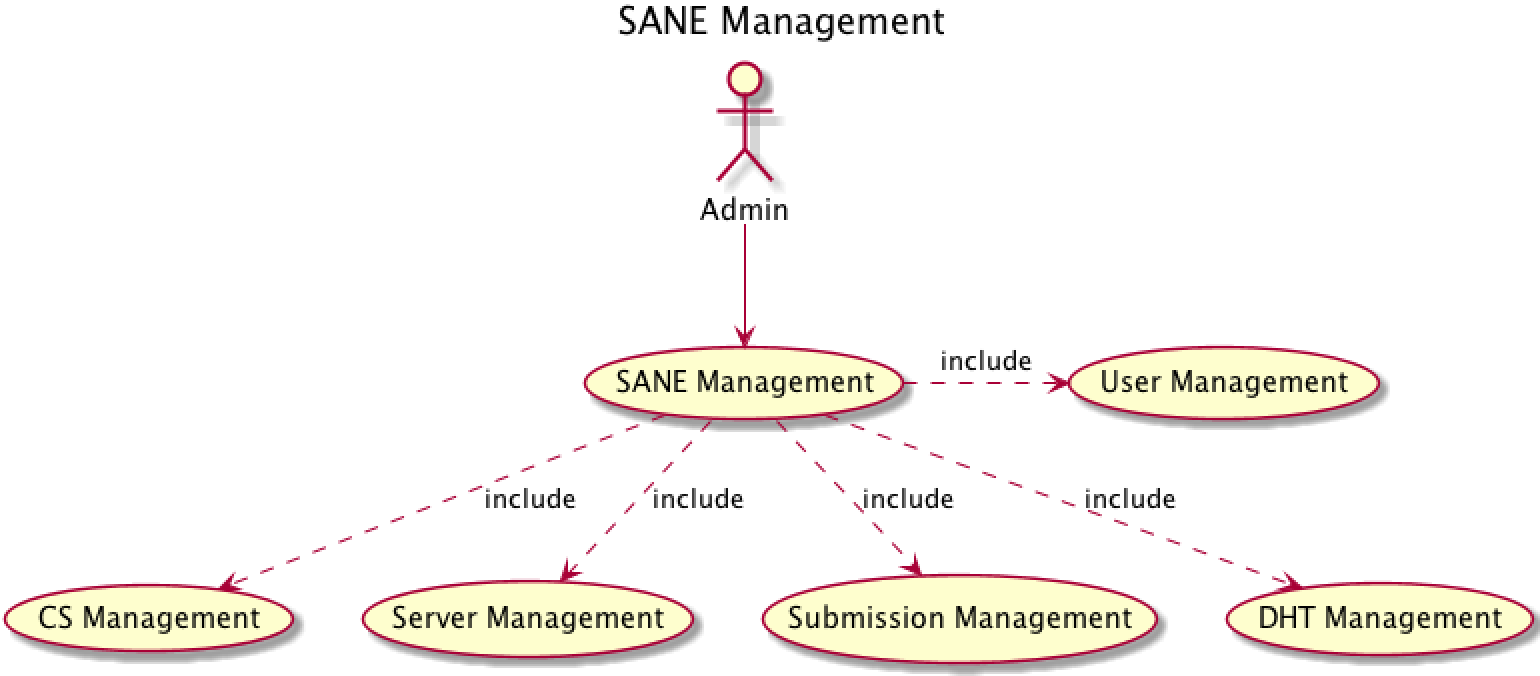
\includegraphics[width=250px, height=100px]{usecase.png}
\caption{use case diagram}
\label{picture-label3}
\end{figure}

Original complete usecase diagram is available in our project folder on Google Drive.

\subsection{\large User Interface Design}
Our project is a web application that enables the administrator to manage SANE node visually. Therefore Graphical User Interface is a critical factor to user experience. GUI must be easy for use, style-consistent. In order to achieve compatibility between desktop and mobile devices, responsive layout has been applied at frontend of our project. This will promote user experience greatly. We have used Mockups as the prototype design tool for GUI at the beginning of the project. Mockups is a awsome prototype design tool for web application that is able to run on different platforms, e.g. Windows, Linux, FreeBSD, Mac OS, etc. Mockups also supports online/offline mode. Therefore we could construct a web application prototype in a short time to instruct our future development effectively.Figure 4 is user view prototype and figure 5 is statistical diagram of device view:\\\\
\begin{figure}[htb]
\centering
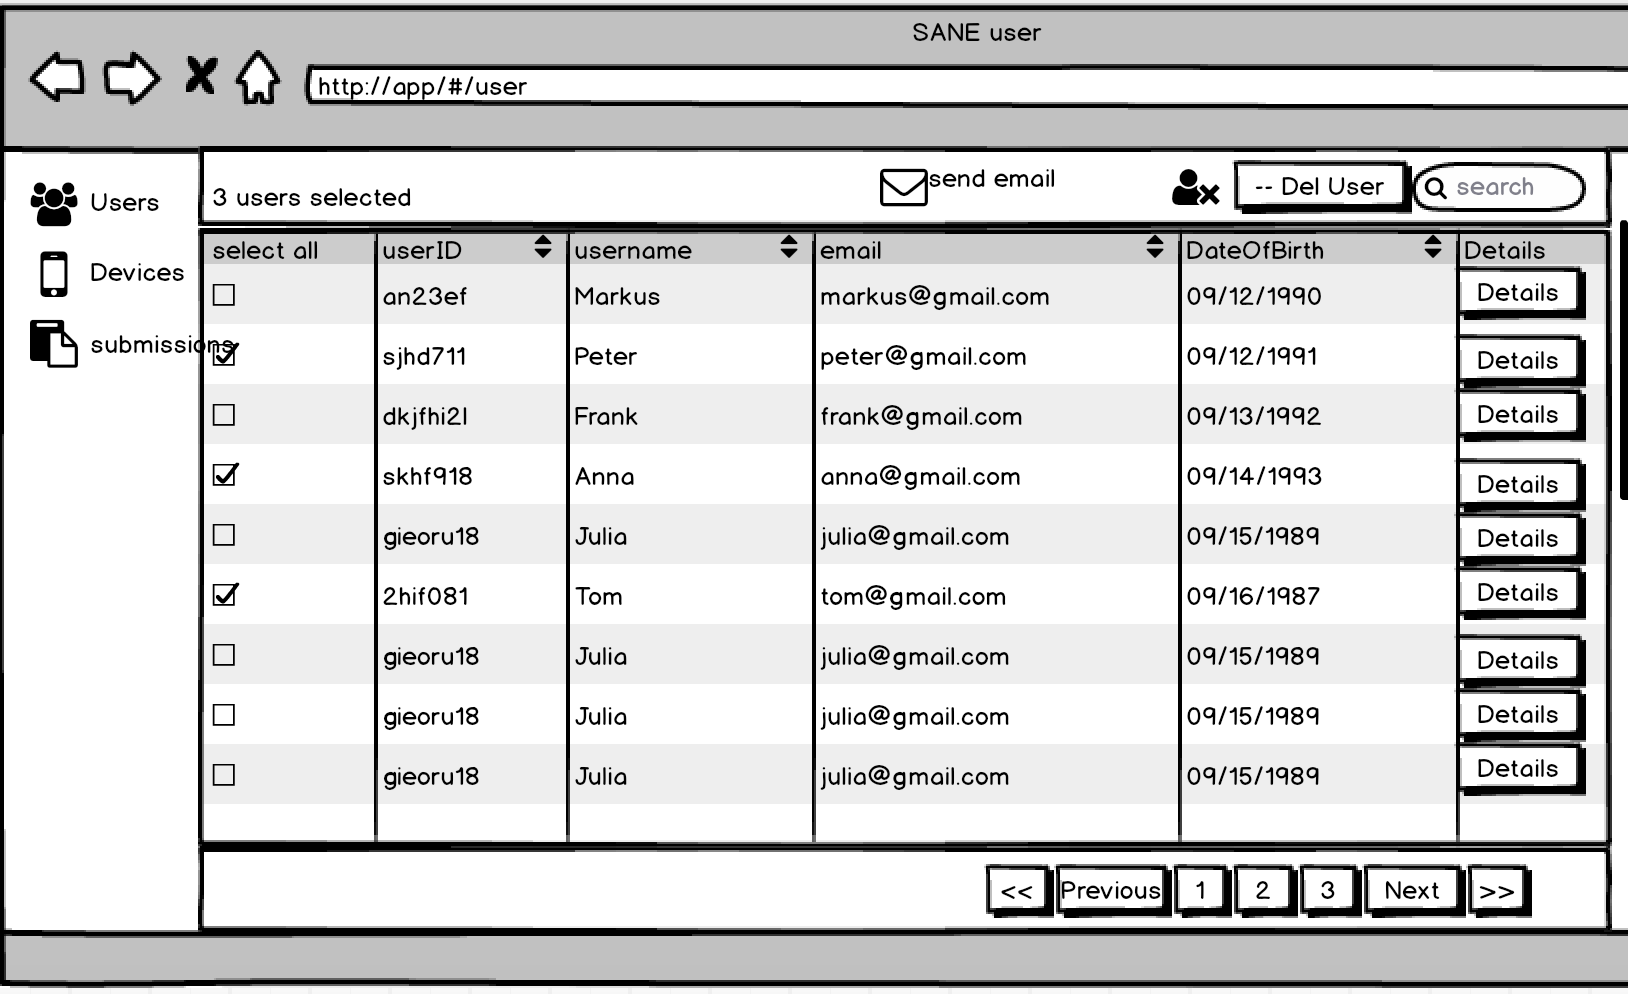
\includegraphics[width=250px, height=120px]{gui.png}
\caption{Prototype User View}
\label{picture-label4}
\end{figure}
\begin{figure}[htb]
\centering
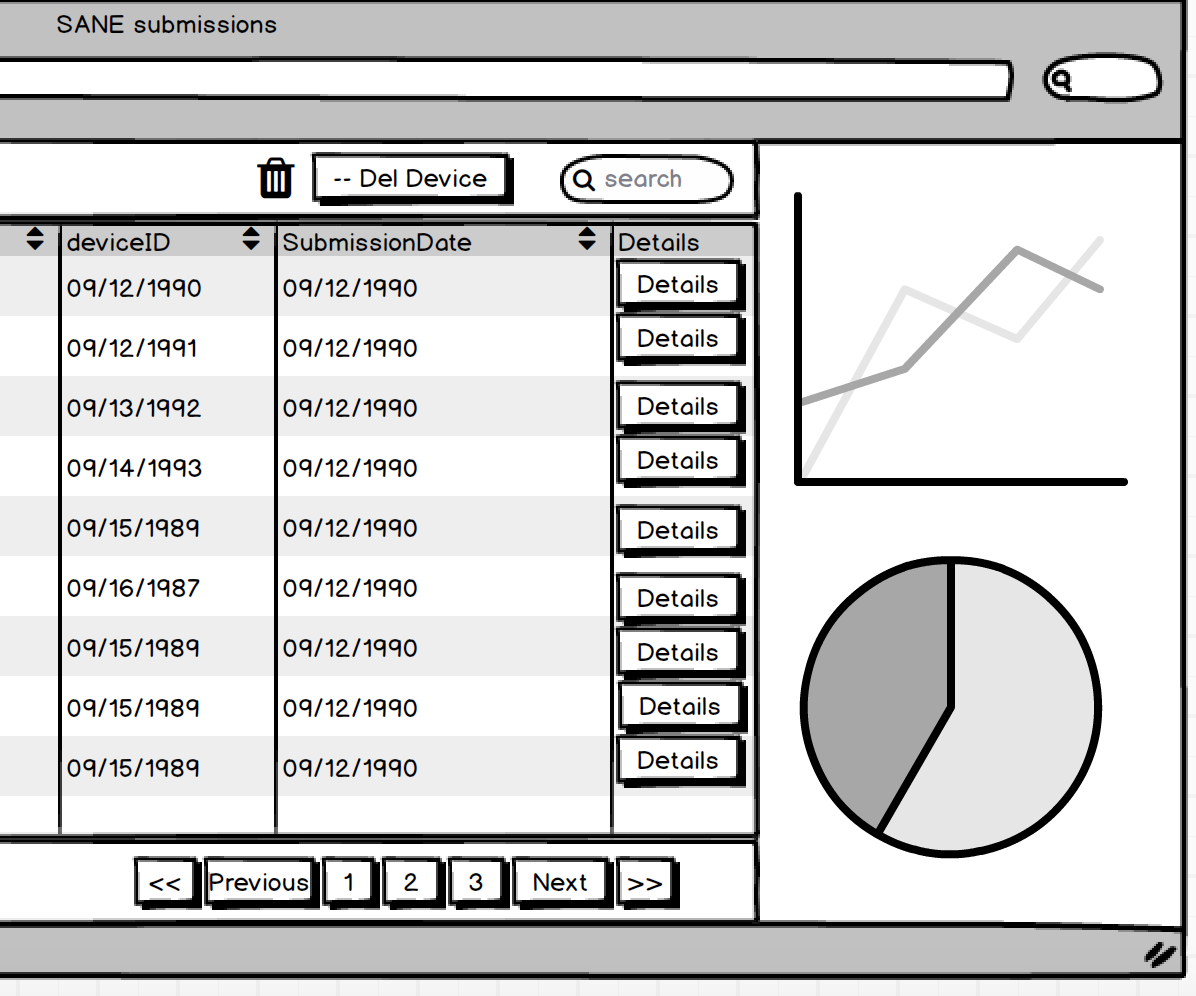
\includegraphics[width=250px, height=120px]{device.png}
\caption{Prototype Statistical Diagram of Device view}
\label{picture-label5}
\end{figure}
Original complete mockups prototype is available in our project folder on Google Drive.

\subsection{\large RESTful API Negotiation}
We choose RESTful API to provide data for front-end of our system. REST(Representational State Transfer) is a kind of architectural style or design style, but not a concrete standard. All of the Resources could be identified by Uniform Resource Identifiers. RESTful systems typically, but not always, communicate over Hypertext Transfer Protocol (HTTP) with the same HTTP verbs (GET, POST, PUT, DELETE, etc.) that web browsers use to retrieve web pages and to send data to remote servers. RESTful API is widely applied in client-server architectural software to achieve loosely coupled systems. Front-end could be easily separated from back-end, both sides could be developed independently. This benefit has been proven by our later development.\\\\
The RESTful APIs have been published formally using swagger as a extension of Flask web framework. This tool will be introduced later in Technology Selection subsection. The request message format and the return value format have been negotiated and defined before development. Following figures show the RESTful APIs and message format of some APIs. The complete protocol is available both in file ``API\_Specs.md'' and on http://127.0.0.1:5000/api/spec.html\\
\begin{figure}[htb]
\centering
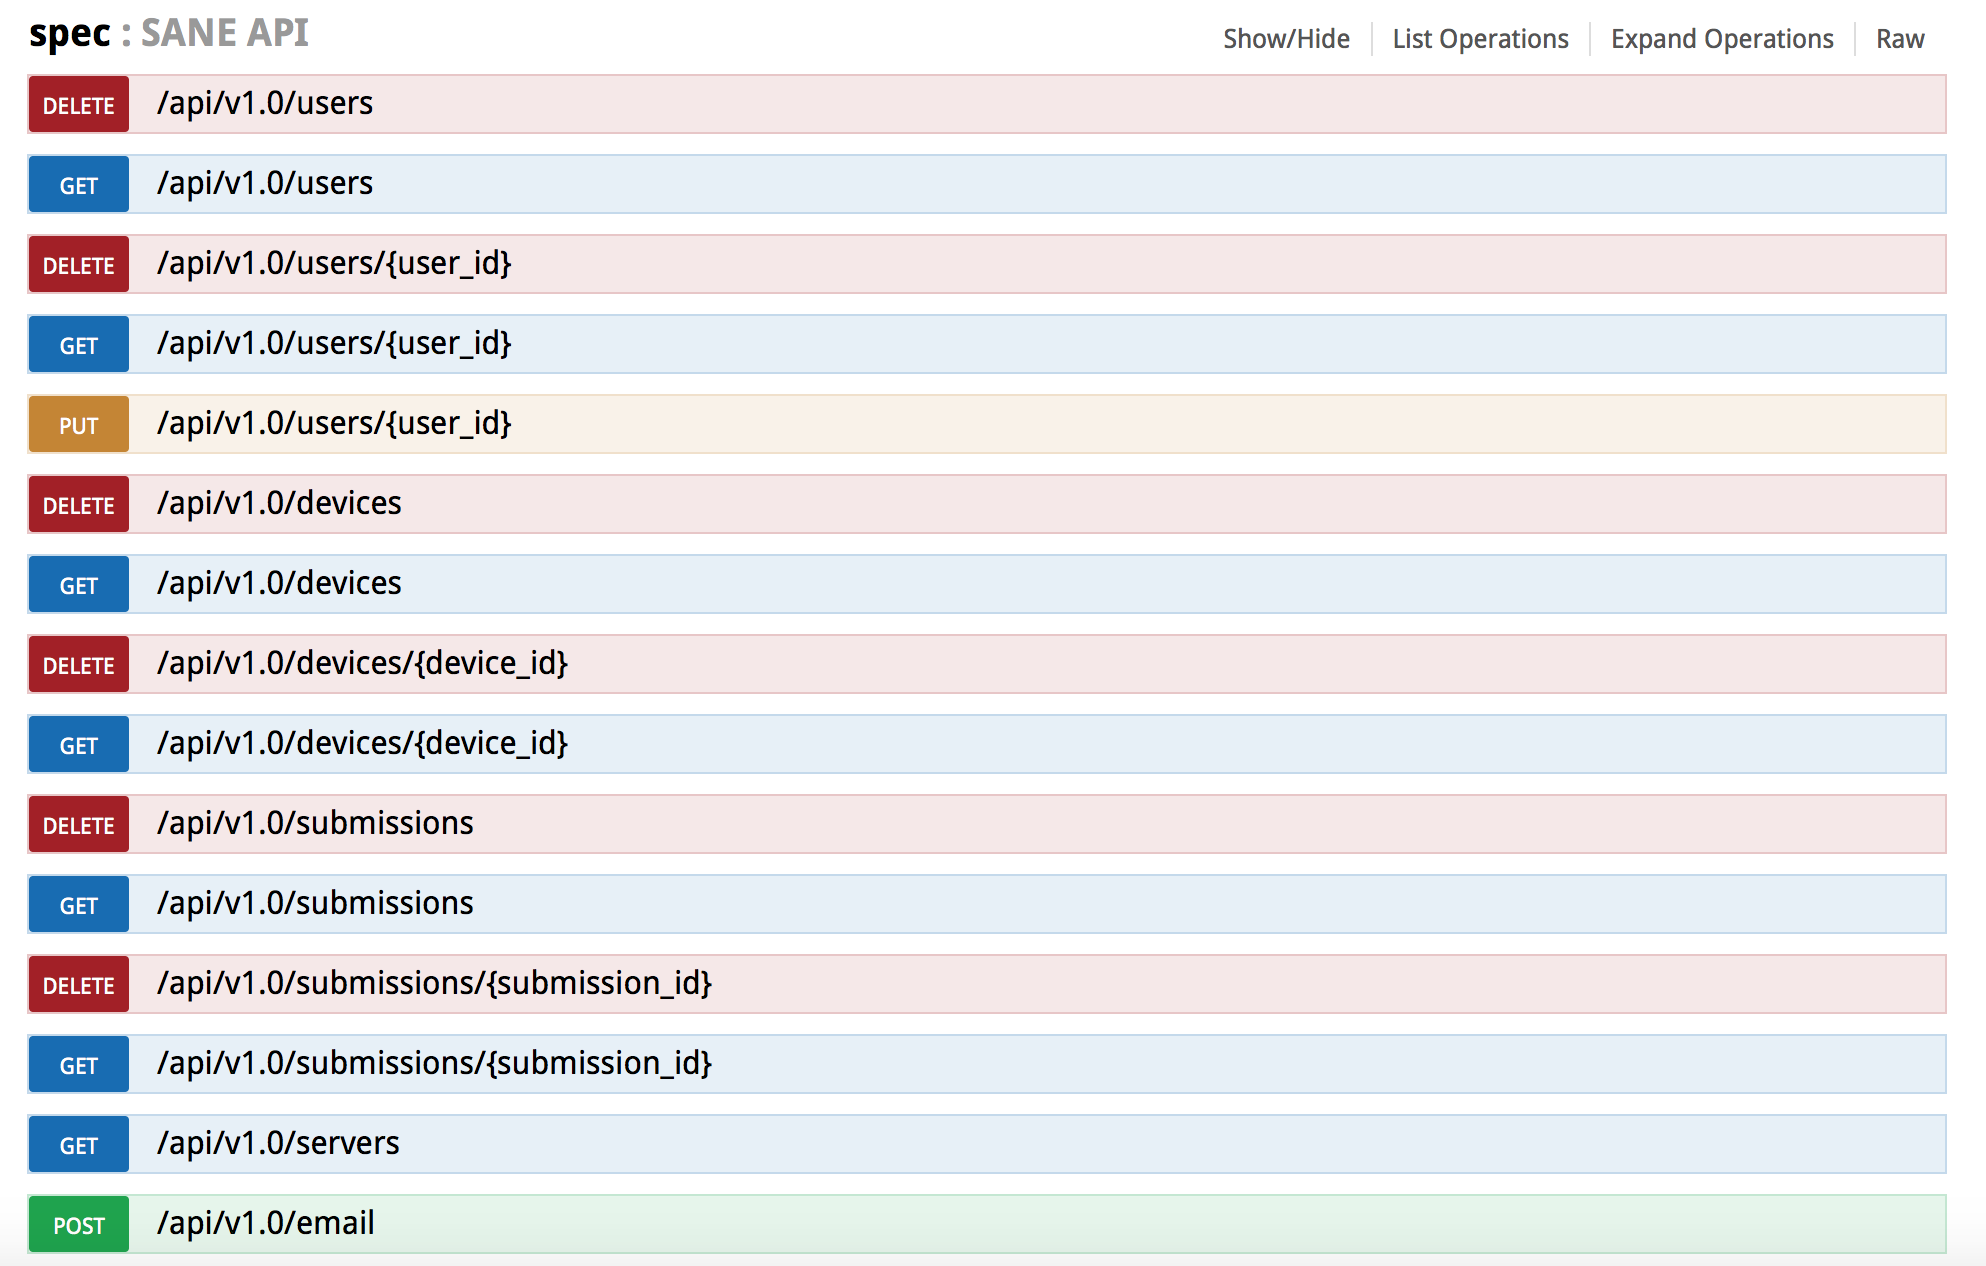
\includegraphics[width=250px, height=120px]{api.png}
\caption{API Overview}
\label{picture-label6}
\end{figure}
\begin{figure}[htb]
\centering
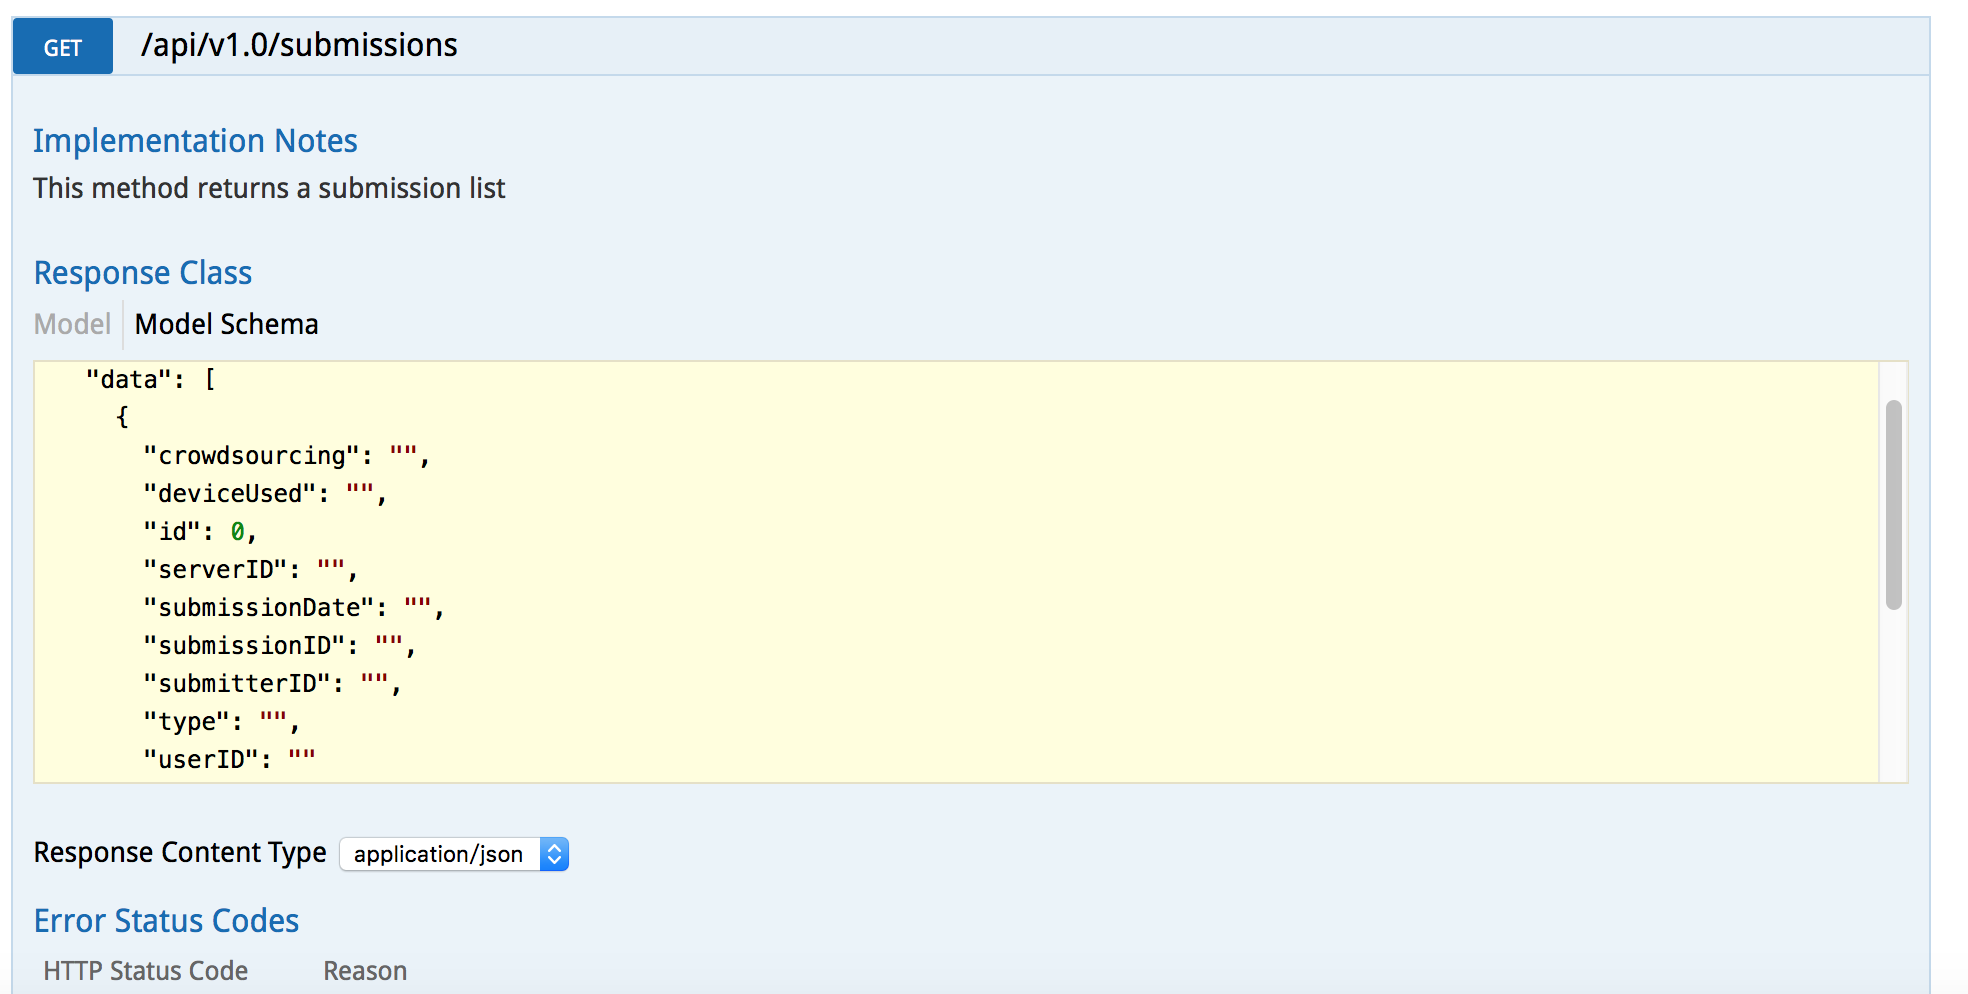
\includegraphics[width=250px, height=120px]{api2.png}
\caption{Model Schema}
\label{picture-label7}
\end{figure}

\subsection{\large Technology Selection}
Our system mainly consists of three layers, namely frontend presentation layer, business-logic layer, persistence layer. Backend is responsible for most of the heavy lifting and integration work of our product. It handles data persistence, retrieval, caching, relationship, email delivery, user management, cookie, session, etc. Frontend is responsible for presentation and virtual management. Frontend is somehow like single page application, e.g. Gmail. We use NPM(node package management) to manage our tools at frontend. NPM is the package management tool on Node.js. Install, Uninstall, Update, Query, Distribution of Node.js package could be completed automatically. NPM has liberated programmer from heavy package management. Programmers are able to focus on development of product features. The best way to apply NPM is to create a package.json file. This file has afforded us lots of good things. We didn't have to install a package step by step. What we need to do is to write a package record to package.json. Furthermore, package.json allows us to specify the version of a package. Package.json helped sharing of package between different developers a lot.\\\\ 
Gulp and Bower were installed automatically using NPM. Gulp is a Node.js-based frontend tool for development and deployment automation. It's not only capable of optimizing website resources, but also automating many repetitive tasks during development. There is a file gruntfile.js, where we could define our tasks, in JavaScript or CoffeeScript. e.g. linking JavaScript and CSS, parsing templates, compiling LESS.\\
Figure 8 shows a script snippet of self-defined gulp tasks:\\
\begin{figure}[htb]
\centering
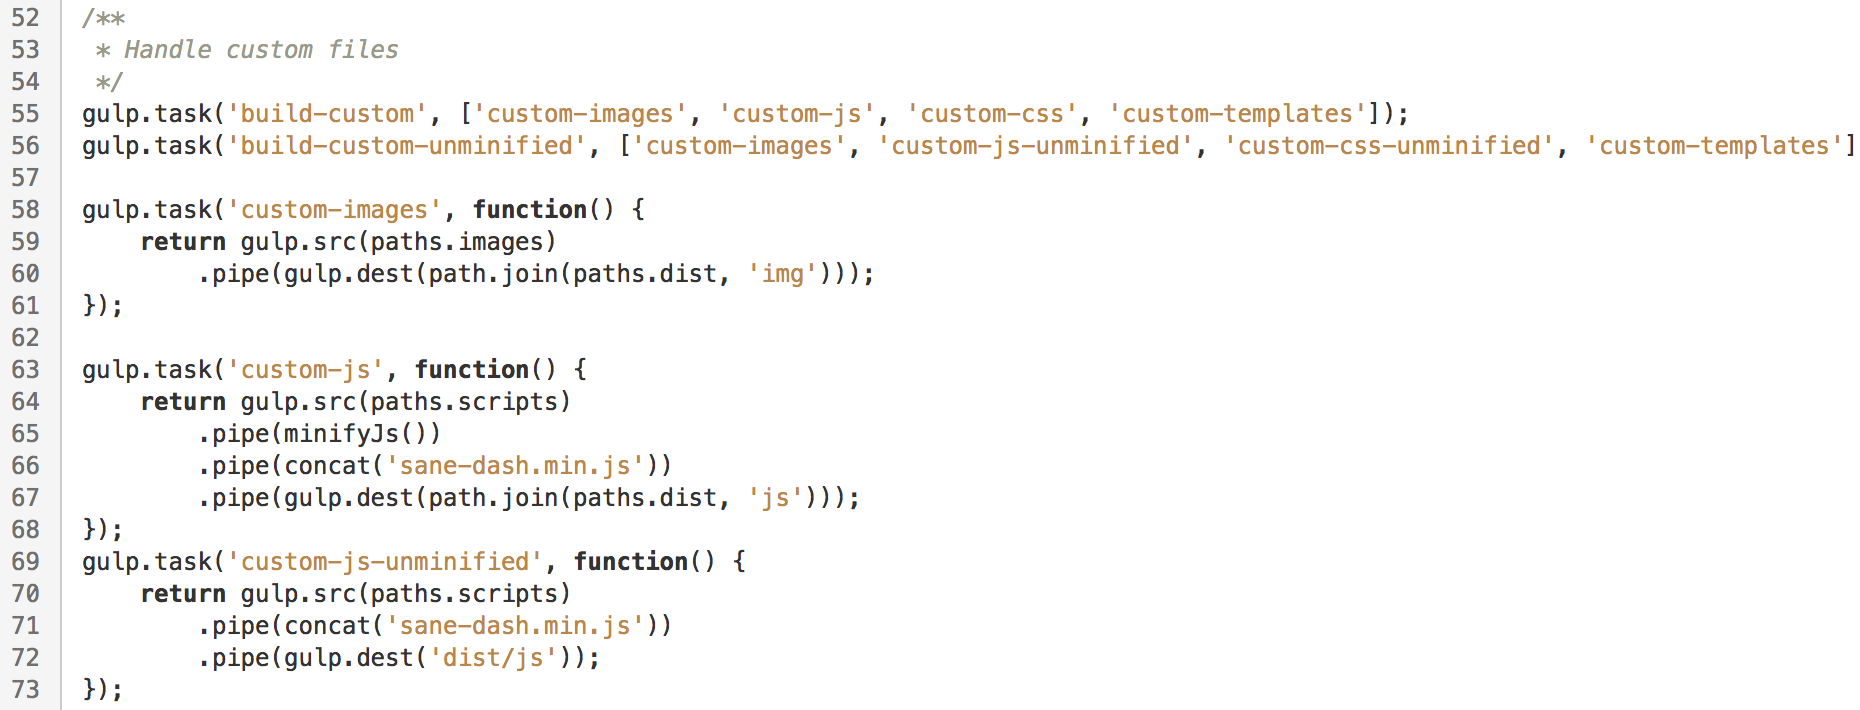
\includegraphics[width=250px, height=120px]{gulp.png}
\caption{Gulp Tasks}
\label{picture-label8}
\end{figure}

Bower is a opensource package management tool for frontend development developed by twitter. It enables automatic installation of JavaScript and CSS dependencies. Bower and NPM overlap in functionality to some extent. Nowadays NPM was known not only as Node Package Management, but also as JavaScript Package Management. This means, NPM could  be applied both in frontend and backend development. NPM supports nested dependency, this means, each package might have its own subdependencies. This is really great on the server where you don't have to care much about space and latency. But one obvious drawback is that multiple copies of the same dependencies in different versions may be downloaded. We used Bower as our frontend package management due to its flat dependency tree. Bower requires only one version for each package to reduce page load to a minimum. We just need to write a dependency into bower.json file. The package will be installed automatically.Figure 9 shows a snippet of bower.json:\\
\begin{figure}[htb]
\centering
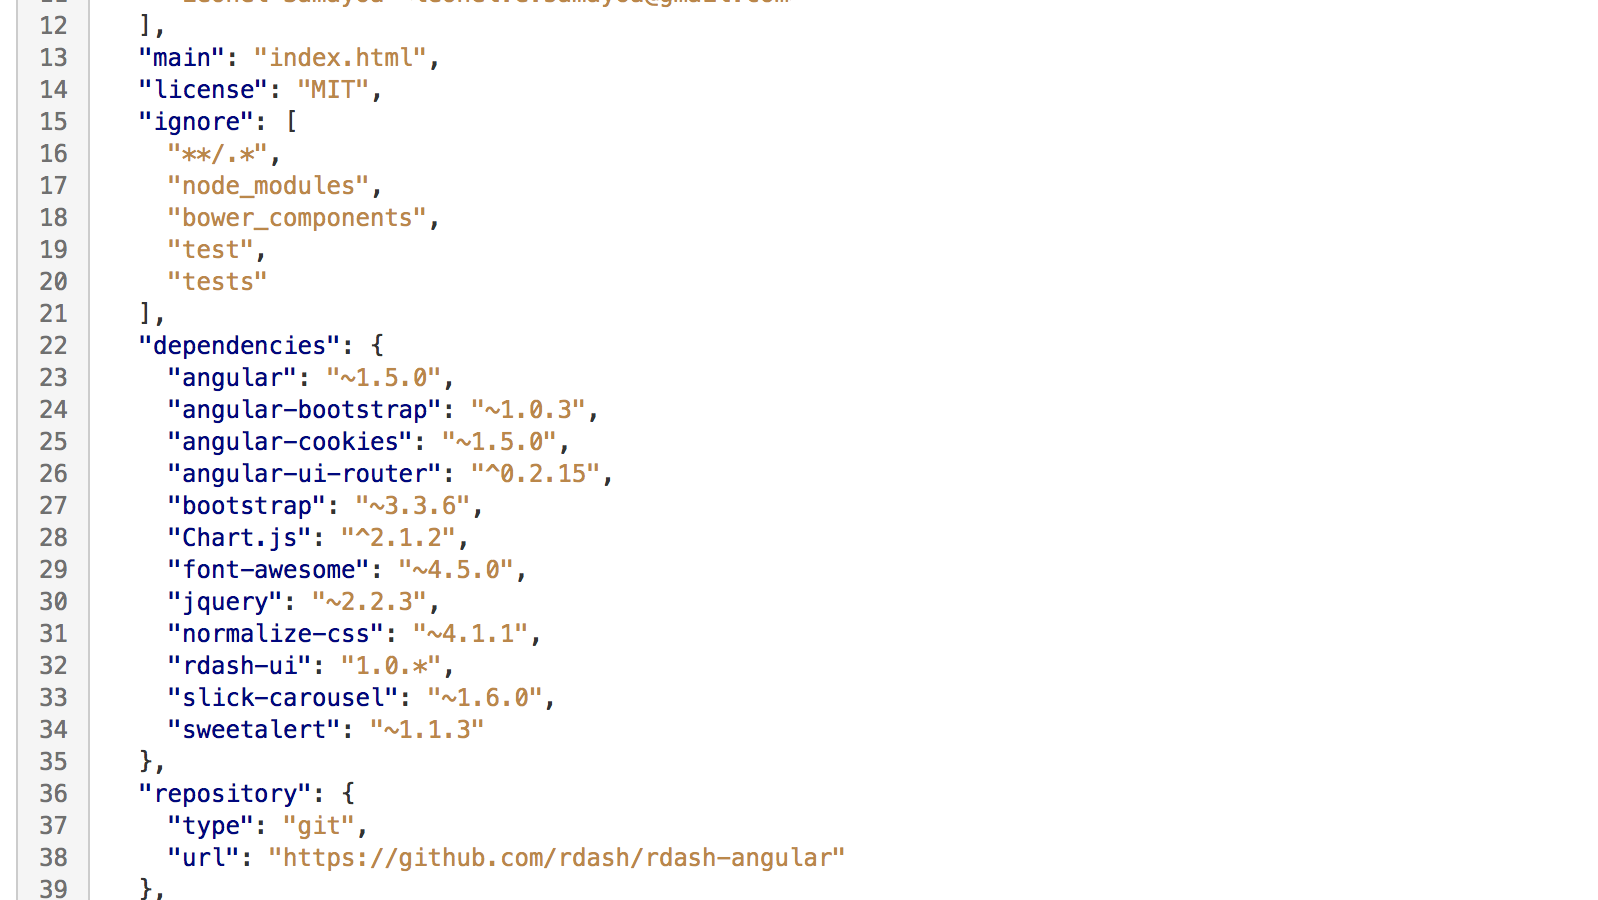
\includegraphics[width=250px, height=120px]{bower.png}
\caption{bower.json}
\label{picture-label9}
\end{figure}\\
Bootstrap comes from Twitter, it is a very popular front-end framework currently.Bootstrap is built on HTML, CSS, JAVASCRIPT , it is simple and flexible, so that Web development has been greatly simplified. Bootstrap contains a wealth of Web components,with these components, we could quickly build a beautiful, fully functional website. Bootstrap has been applied to build our frontend UI and responsive layout. Desktop client and mobile client could be perfectly compatible with each other.\\\\
AngularJS was developed by Misko Hevery in 2009 and then purchased by Google to address many of the challenges encountered in developing single-page applications. AngularJS provides many awesome features, e.g. client-side model–view–controller (MVC), model–view–viewmodel (MVVM), Two-way Data Binding. AngularJS  presents a higher level of abstraction to simplify application development. Like other abstract technology, angularjs will also lose some flexibility. In other words, AngularJS is not suitable for all applications. It is mainly used to build CRUD applicaiton. Fortunately, at least 90\% of WEB applications are CRUD applications. Our project is no exception.\\
\begin{figure}[htb]
\centering
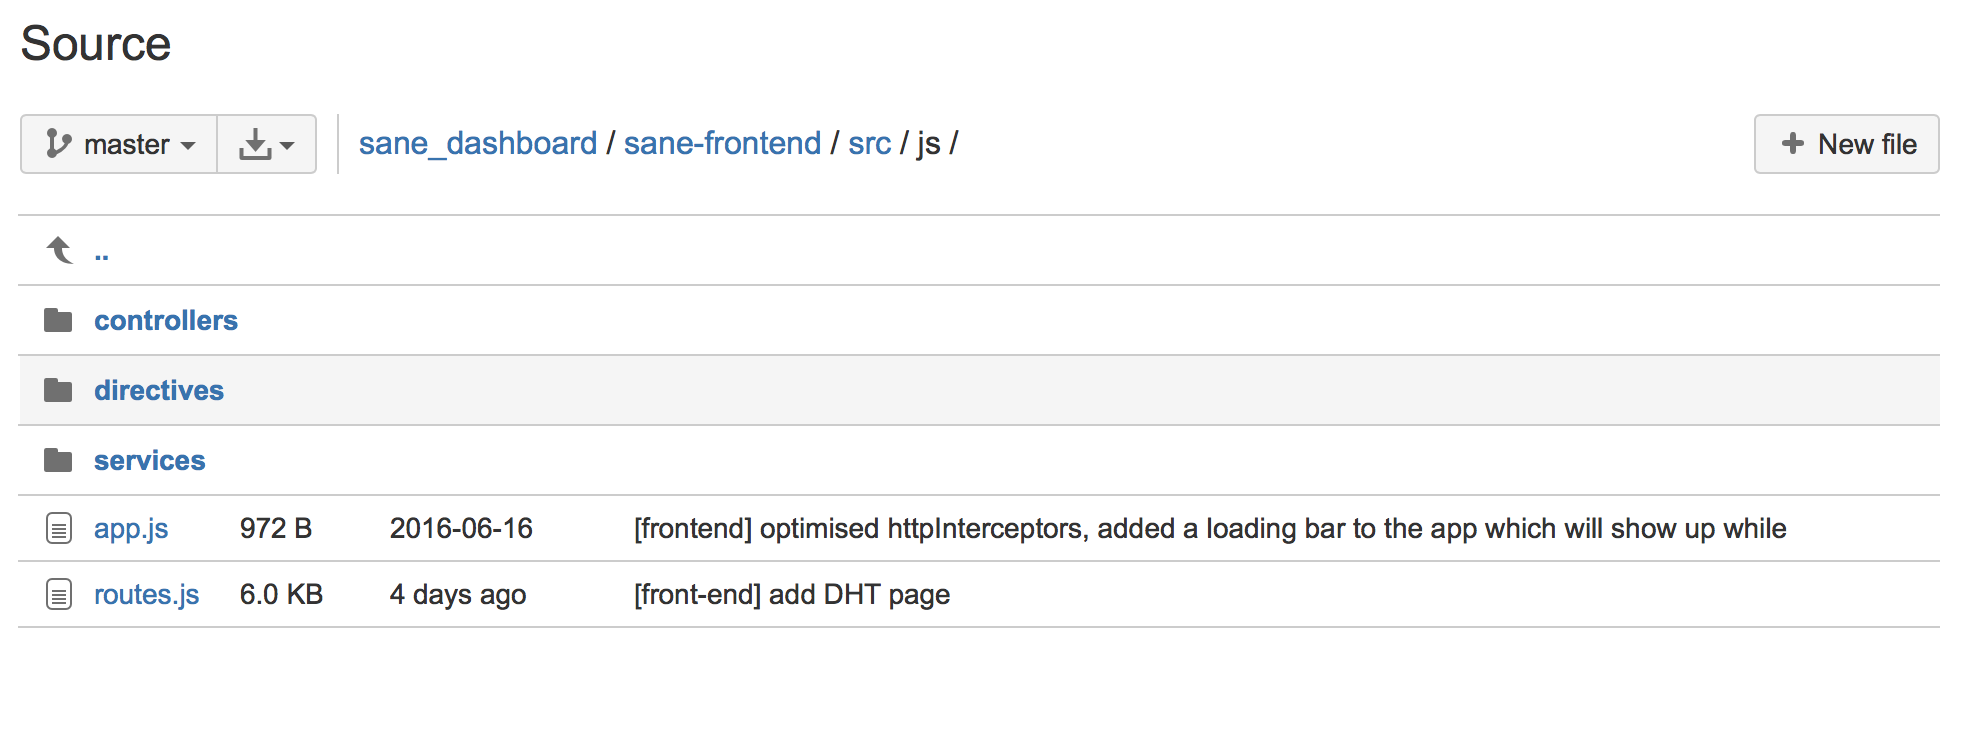
\includegraphics[width=250px, height=120px]{angular.png}
\caption{Frontend Route MVC}
\label{picture-label10}
\end{figure}\\
Chart.js is a HTML5-based chart library that uses the canvas element to show a wide range of client charts, line charts, bar charts, radar charts, pie charts, ring maps. In each chart, it contains a large number of customization options, including animated display format. Chart.js relatively lightweight (gzip version only 4.5k), and does not depend on other libraries. In our project, Chart.js is used to draw statistical results of SANE node, including registered user distribution, age distribution, education registration, etc.\\
\begin{figure}[htb]
\centering
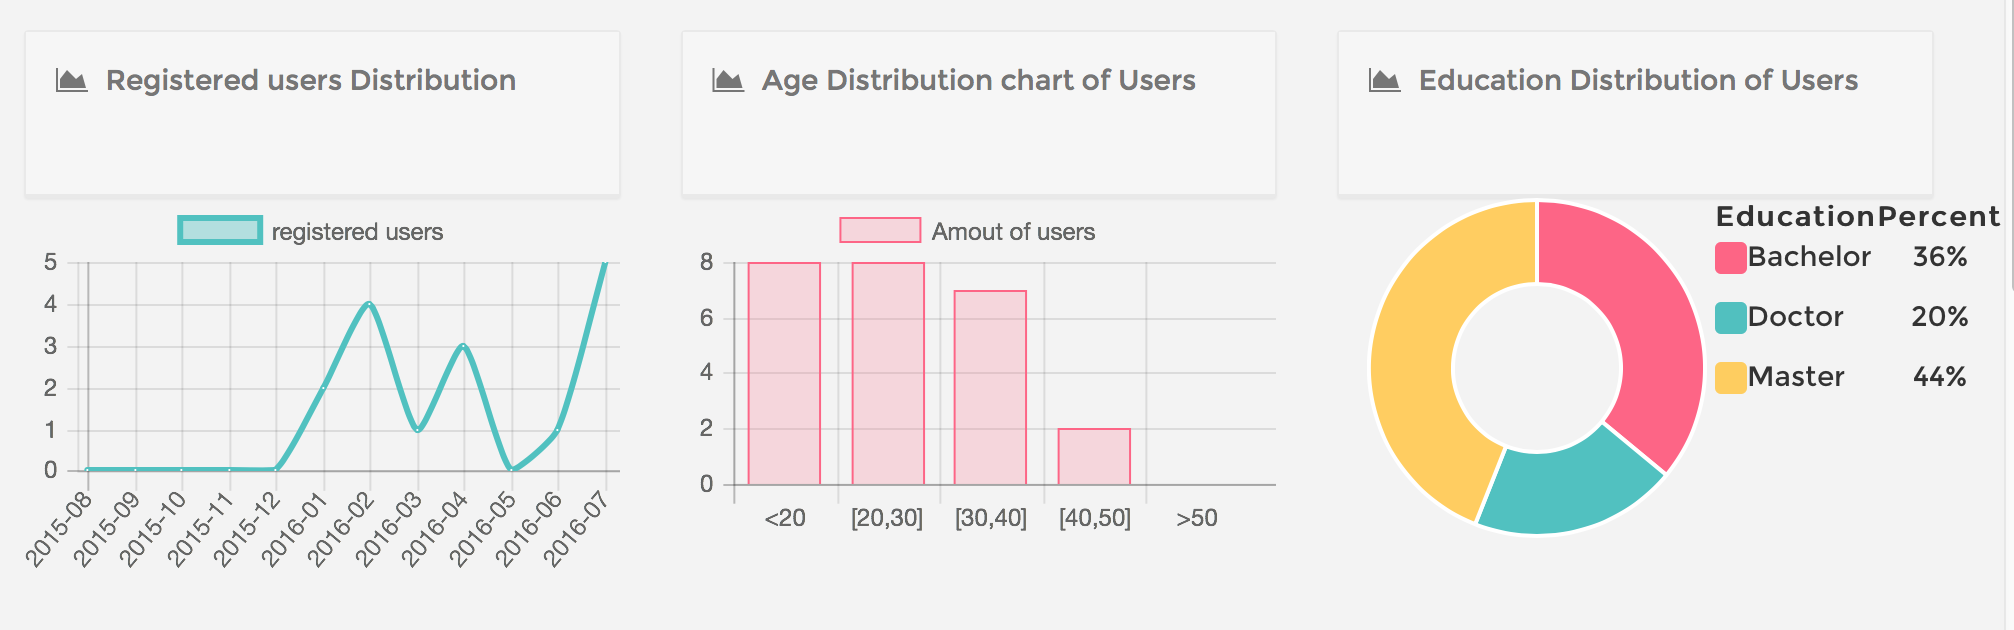
\includegraphics[width=250px, height=120px]{chartjs.png}
\caption{Chart.js}
\label{picture-label11}
\end{figure}\\
We applied Python as programming language in backend. Python is very easy to learn, it has a simple and elegant syntax. Usually code in Python that provides some features is much simpler than other languages. This means, the development cycle could be largely shortened.\\\\
Because of teamwork, we had to unify our development environment, including Python version, dependencies versions. Pyenv is a Python version management tool that enables coexistence of multiple versions and allows user to switch Python versions easily. This affords us a development version of Python without affecting system Python environment. We used Python 2.7.11 as the development version.\\\\
Dependency management is a critical factor that affects teamwork greatly. Pip is a popular package management tool of Python. Many packages can be found in the Python Package Index (PyPI). Pip support management of a full list of packages through a ``requirement'' file.  This enables the efficient recreation of the original packages in a new environment. The command looks like ``pip install -r requirement.txt''. But pip is only responsible for dependency management, it has no concern about project build and deployment. We need a tool like Maven of Java that permits automatic project build and deployment as well as dependency management. zc.buildout has fulfilled these tasks. Buildout is a tool developed by Zope Corporation's JimFulton that aims to create cross-platform reusable program. Buildout could build, compose, deploy an application from multiple parts through a configuration file ``buildout.cfg''. Buildout could not only automatically install, update dependencies like setuptools , but also construct a separate environment like virtualenv. Figure 12 shows a script snippet of our buildout.cfg file:\\
\begin{figure}[htb]
\centering
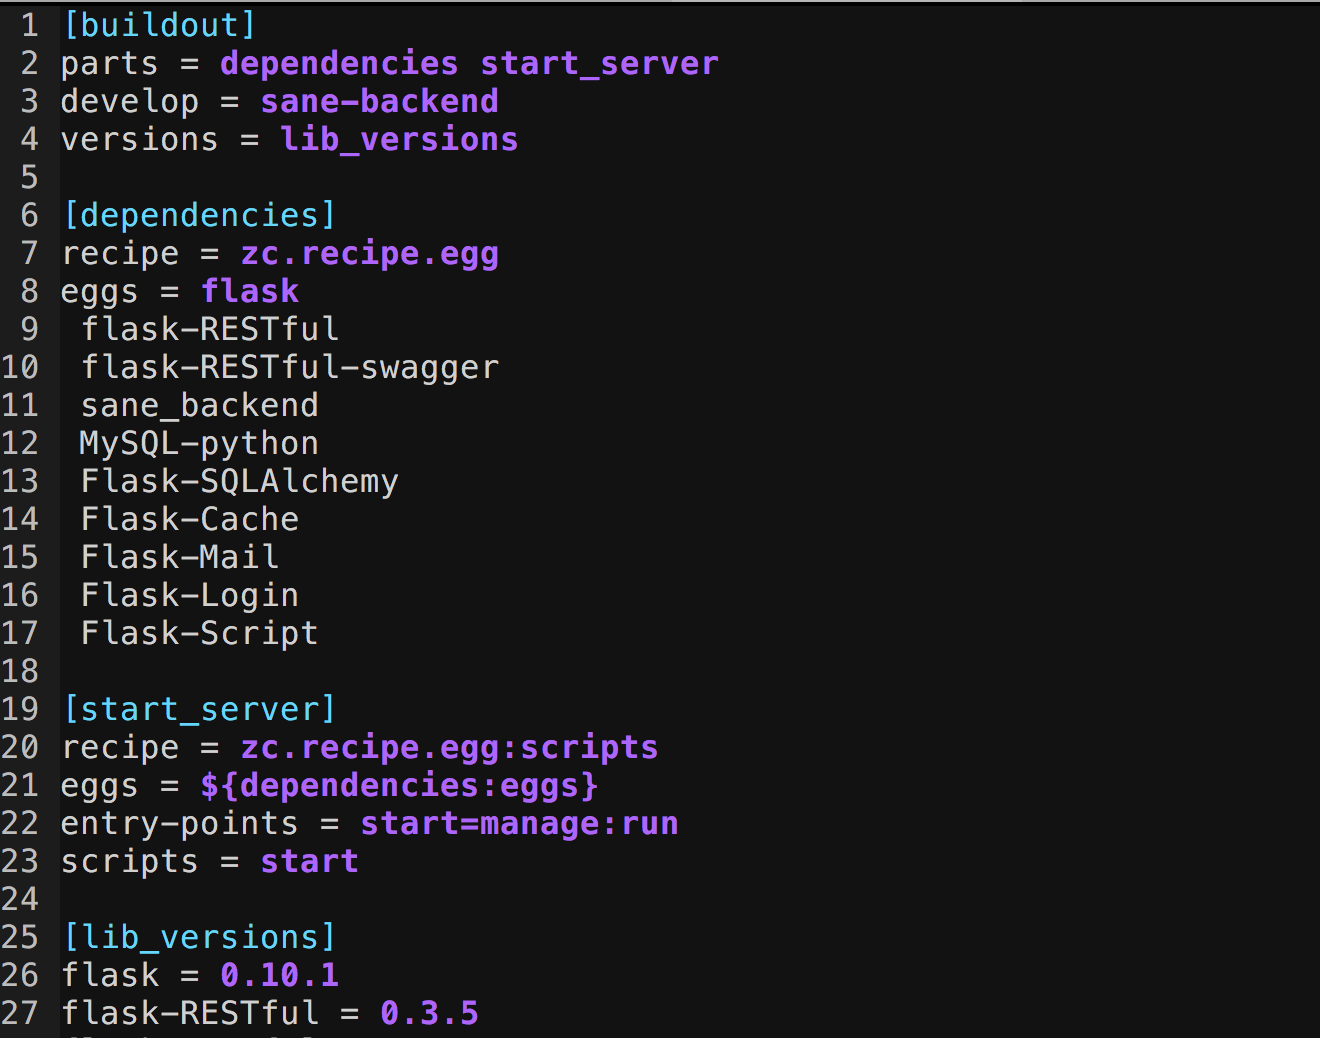
\includegraphics[width=250px, height=120px]{buildout.png}
\caption{buildout.cfg}
\label{picture-label12}
\end{figure}\\
Our project is a web application. The world of Python web frameworks is full of choices. Django, Flask, Pyramid, Tornado, Bottle, Diesel, Pecan, Falcon, and many more are competing for developer mindshare. It seems like that Django dominates the world of Python web. Django is a high-level Python Web framework that encourages rapid development and clean, pragmatic design. Django consists of a wide range of solutions for almost all fields in web development, e.g. template engine, ORM, form, route distribution, login, cookie, session, etc. Community of Django, both official and unofficial(Stackflow and IRC) community are very active. Basically any problems we encountered will have mature solutions.\\\\
Flask is just the opposite of Django. Flask is a micro web framework written in Python and based on the Werkzeug toolkit and Jinja2 template engine. It is BSD licensed. Flask framework itself contains only routing distribution, request/response encapsulation, plugin system, Werkzeug(process WSGI), Jinja2(template engine) and Flask-SQLAlchemy extension(Model layer). These form a complete MVC framework. For Flask itself, a micro- framework, it was enough, it can only provide so much. If more additional features are needed, we just need to extend Flask by Flask plugins, namely extensions of Flask. If we need to process forms, just install Flask-WTF, if we need login authentication, just install Flask-Login, if we need Administration, just install Flask-Admin. Due to the lightweight of Flask, we used Flask as our web framework.\\\\
Basically our project is a CRUD web application. Database access is a basic feature. We chose SQLALchemy as our ORM(Object Relation Mapping) framework. Despite strong influence of Django SQLAlchemy is de facto standard of ORM framework in the world of Python. SQLAlchemy has been widely used in the next generation Python Web framework built on WSGI standard. One advantage of using SQLAlchemy is that it permits developers to first consider the data model, and then decide later visual data mode(using the command-line tool, Web GUI framework or frame).\\\\
Our backend published RESTful API for frontend. This means, backend and frontend could be developed simultaneously. Flask Framework is capable of publishing RESTful service. A sample of Flask published API looks like the following:\\\\
\scriptsize{\textbf{\emph{from flask import abort\\
@app.route(`/todo/api/v1.0/tasks/$\langle int:task\_id\rangle$', methods=['GET'])\\
def get\_task(task\_id):\\
\_\_\_\_task = [task for task in tasks if task[`id'] == task\_id]
\_\_\_\_if len(task) == 0:\\
\_\_\_\_\_\_\_\_abort(404):\\
\_\_\_\_return jsonify({`task': task[0]})}}}\\\\
\normalsize{But we chose Flask-RESTful as our extension instead of native Flask. Flask-RESTful simplifies creation of RESTful service and it encourages best practices with minimal setup. A sample of Flask-RESTful looks like the following:\\\\}
\scriptsize{\textbf{\emph{from flask import Flask\\
from flask.ext import restful\\
class HelloWorld(restful.Resource):\\
\_\_\_\_def get(self):\\ 
\_\_\_\_\_\_\_\_return {`hello': `world'}}}}\\\\
\normalsize{After the API on server side completed, we should inform clients how the API could be used, how are the details of API. We chose Flask-RESTful-Swagger as our RESTful API tool instead of maintaining a single document manually. The obvious shortcoming of the latter approach lies in that it is difficult to maintain the accuracy of all documents, as the server-side API updates. We have to make extra effort to track changes of API. Swagger makes it easy to publish RESTful API with projects. It supports many popular programming language including Python. Flask-restful-swagger is a wrapper for Flask-RESTful which enables swagger support. In essense, we just need to wrap the API instance and add a few python decorators to get full swagger support.\\\\
Usually during the development of RESTful service, we must consider the cache to improve the performance of service. We chose Flask-Cache as our extension for caching. If we want to use simple caching for test, the built-in SimpleCache is a good choice. Data will be cached in memory of Python interpreter. If we want more powerful caching system, e.g. memcached, make sure to have one of the memcache modules supported and a memcached server running somewhere. This is how we connect to such an memcached server:\\}

\scriptsize{\textbf{\emph{from werkzeug.contrib.cache import MemcachedCache\\
cache = MemcachedCache(['127.0.0.1:11211'])\\}}}

\normalsize{In our project we used the built-in SimpleCache for caching. If we want to promote performance of data access in the future, it's very easy to switch to other dedicated caching system.\\}

As a web-based management dashboard, administrator must be able to notify users by Email when something happens. Flask-Mail has been applied as our Email module. We could set SMTP in our application and add attachments easily.\\\\
A important task of backend is to provide login related features for frontend, e.g. logging in, logging out, and ``remember me'' for a session or cookie for a long period. Flask-Login provides a nice solution for us. We could integrate these features into out system. But Flask-Login is a little more complex than other extensions.\\\\
We used Bitbucket as our project hosting server and Git as our version control system. Because the original database was not available during development, we had to mock up data according to schema described in ``install.php'' for test. All of data could be accessed on the remote DB server.\\ 

\section{\LARGE Concept}
\subsection{\large Backend Concept}
\small{RESTful API:}\\\\
\scriptsize{\textbf{\emph{GET  /api/v1.0/users \_\_\_}}get all users from database}\\\\
\scriptsize{\textbf{\emph{PUT  /api/v1.0/users/user\_id \_\_\_}}update user specified by userid }\\\\
\scriptsize{\textbf{\emph{DELETE  /api/v1.0/users \_\_\_}}delete users specified by userids}\\\\
\scriptsize{\textbf{\emph{DELETE  /api/v1.0/users/user\_id \_\_\_}}delete user specified by userid}\\\\
\scriptsize{\textbf{\emph{DELETE  /api/v1.0/devices \_\_\_}} delete devices specified by deviceids}\\\\
\scriptsize{\textbf{\emph{DELETE  /api/v1.0/devices/device\_id \_\_\_}} delete device specified by deviceid}\\\\
\scriptsize{\textbf{\emph{GET  /api/v1.0/devices \_\_\_}} get all devices from database}\\\\
\scriptsize{\textbf{\emph{GET  /api/v1.0/devices/device\_id \_\_\_}} get device specified by deviceid}\\\\
\scriptsize{\textbf{\emph{DELETE  /api/v1.0/submissions \_\_\_}} delete submissions specified by submissionids}\\\\
\scriptsize{\textbf{\emph{GET  /api/v1.0/submissions \_\_\_}} get submissions specified by deviceid, userid, serverid}\\\\
\scriptsize{\textbf{\emph{DELETE  /api/v1.0/submissions/submission\_id \_\_\_}} delete submission specified by submissionid}\\\\
\scriptsize{\textbf{\emph{GET  /api/v1.0/submissions/submission\_id \_\_\_}} get submission specified by submissionid}\\\\
\scriptsize{\textbf{\emph{GET  /api/v1.0/servers \_\_\_}} get all crowdsourcing servers}\\\\
\scriptsize{\textbf{\emph{GET  /api/v1.0/servers/server\_id \_\_\_}} get single crowdsourcing server by serverid}\\\\
\scriptsize{\textbf{\emph{POST  /api/v1.0/email \_\_\_}} send email to one or multiple users}\\\\
\scriptsize{\textbf{\emph{GET  /api/v1.0/dht \_\_\_}} get neighbors within K-Buckets}\\\\
\scriptsize{\textbf{\emph{GET  /api/v1.0/admin \_\_\_}} get administrator of this SANE}\\\\
\scriptsize{\textbf{\emph{GET  /api/v1.0/owner \_\_\_}} get owner of this SANE}\\

\small{Objectmodel and Relation in page 14:}\\\\
\small{Package Class Diagram in page 15:}\\\\
\begin{figure}[htb]
\centering
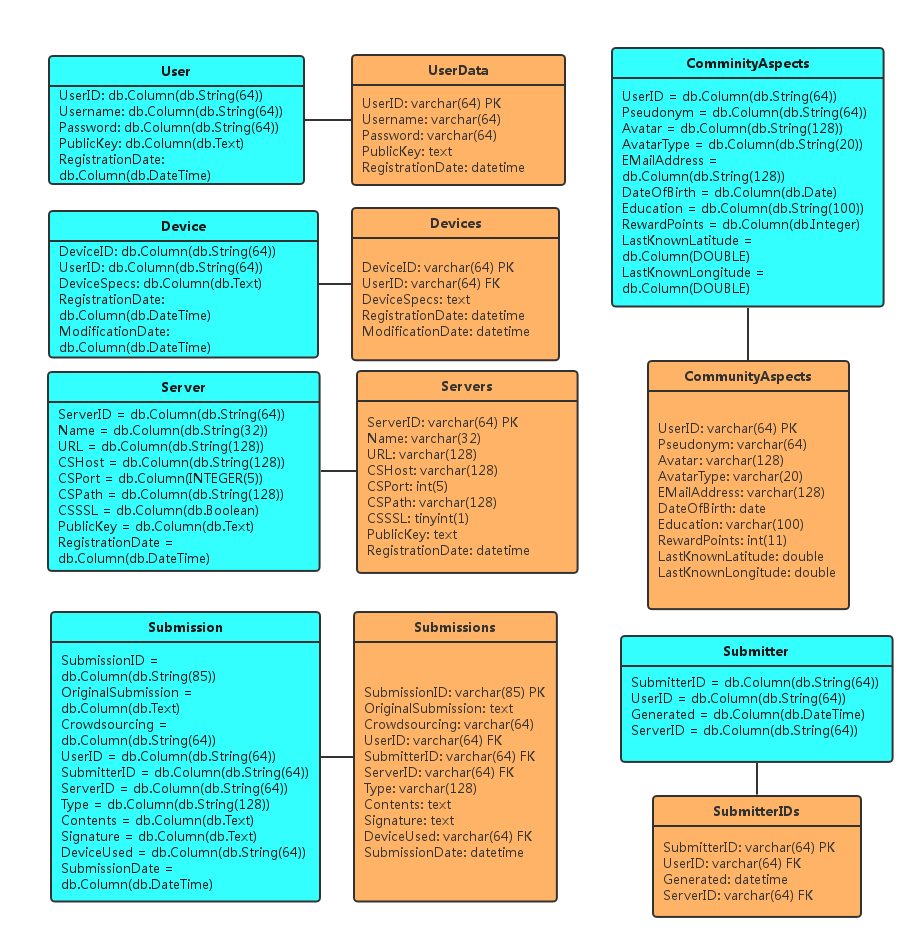
\includegraphics[width=450px, height=550px]{ormd.png}
\caption{Object Relation Mapping}
\label{picture-label13}
\end{figure}\\
\begin{figure}[htb]
\centering
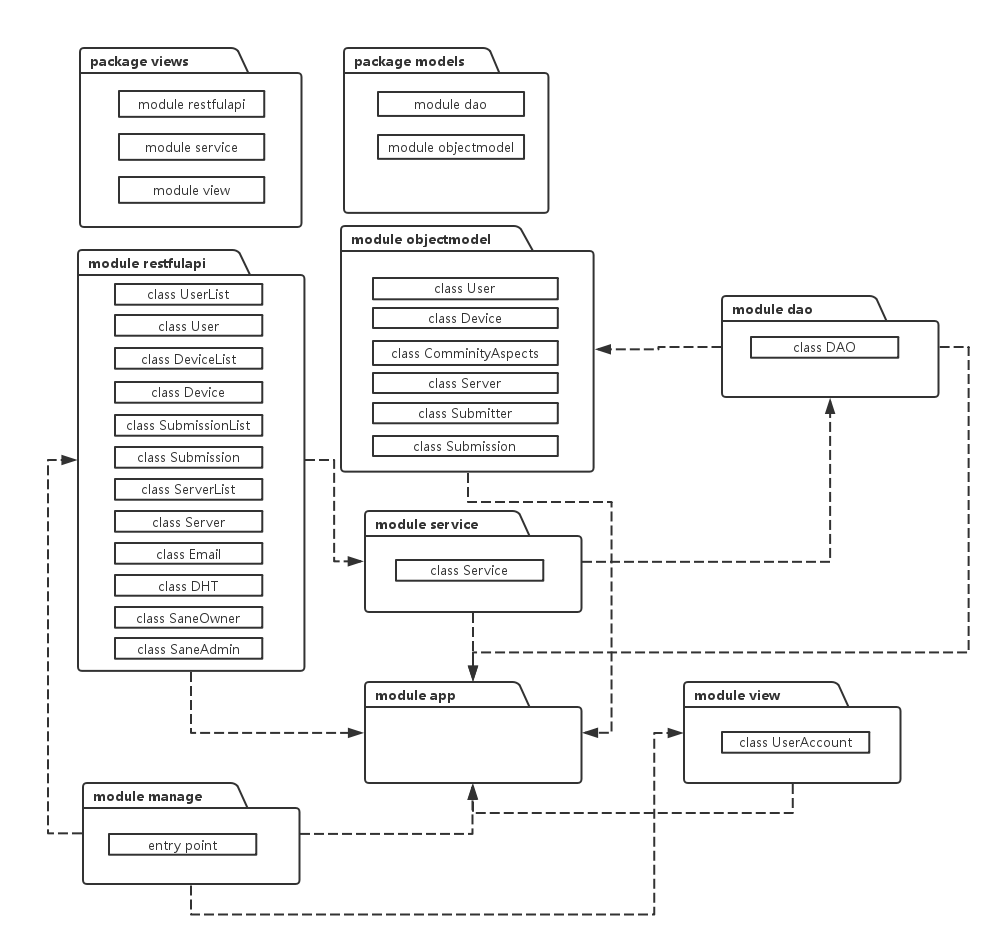
\includegraphics[width=450px, height=550px]{classdiagram.png}
\caption{Package Class Diagram}
\label{picture-label14}
\end{figure}\\
\clearpage
\subsection{\large Frontend Concept}
In frontend, there are some main modules, e.g. Dashboard, Overview, Users, Devices, Submissions, Servers, DHT. Each module is responsible for visualization of an aspect of data stored in SANE. There are two basic views for each module, e.g. user module, there are list view and grid view of users.
\begin{figure}[htb]
\centering
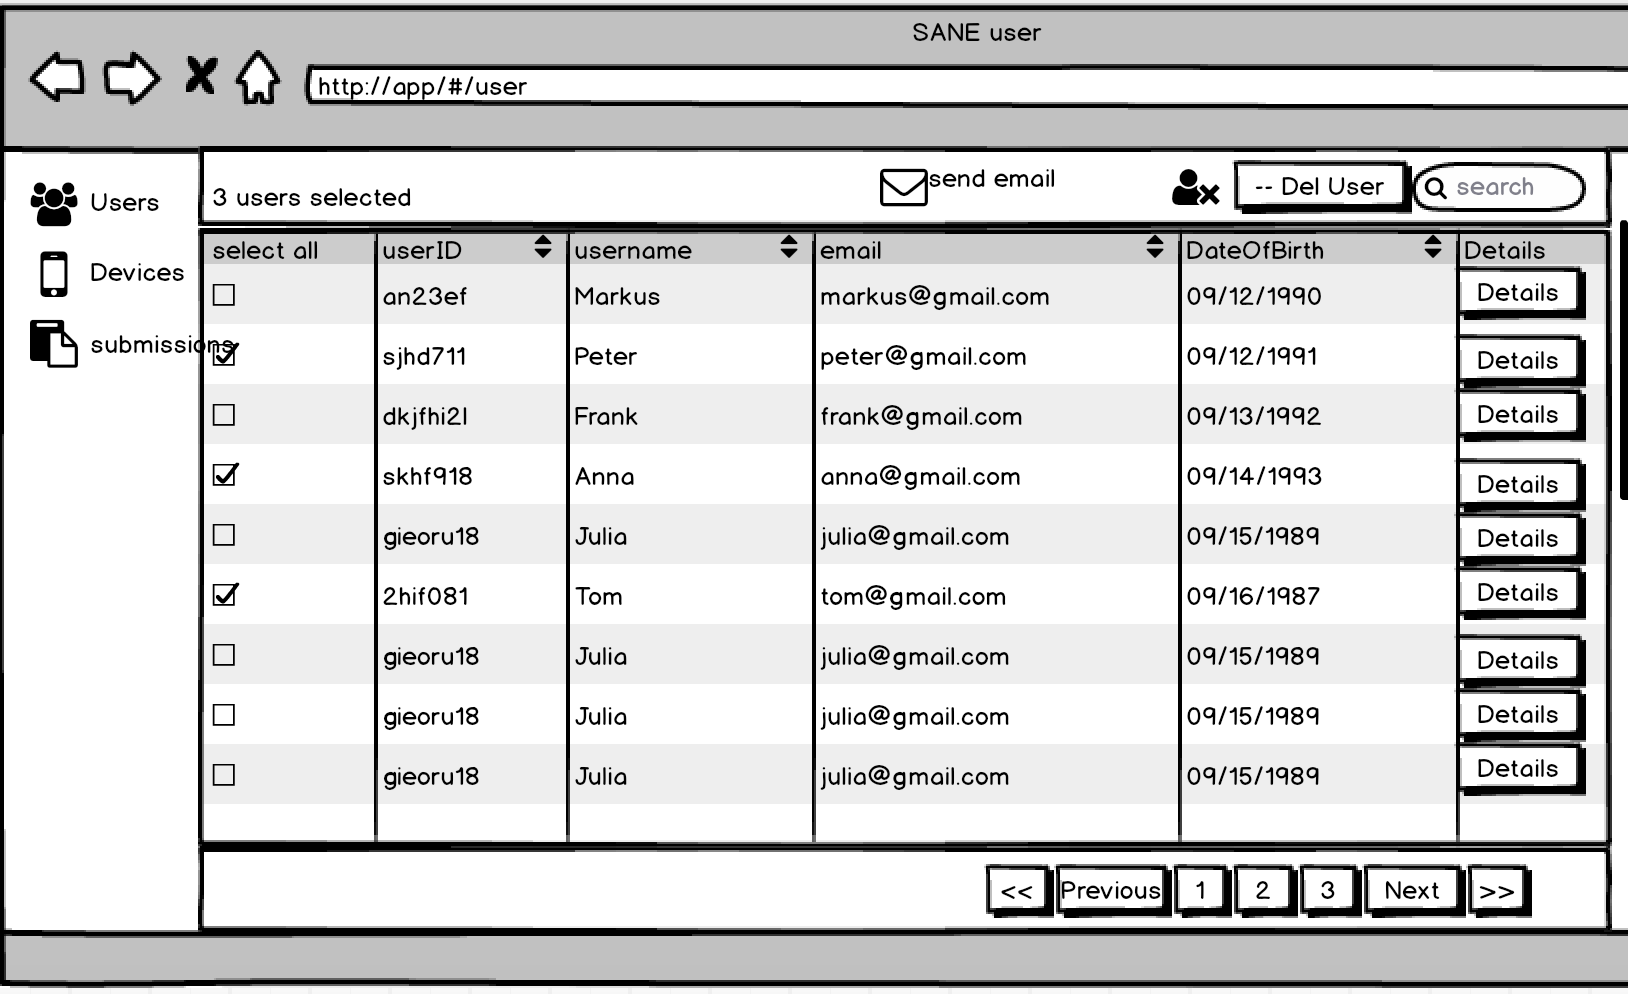
\includegraphics[width=250px, height=120px]{gui.png}
\caption{List View of User}
\label{picture-label15}
\end{figure}
\begin{figure}[htb]
\centering
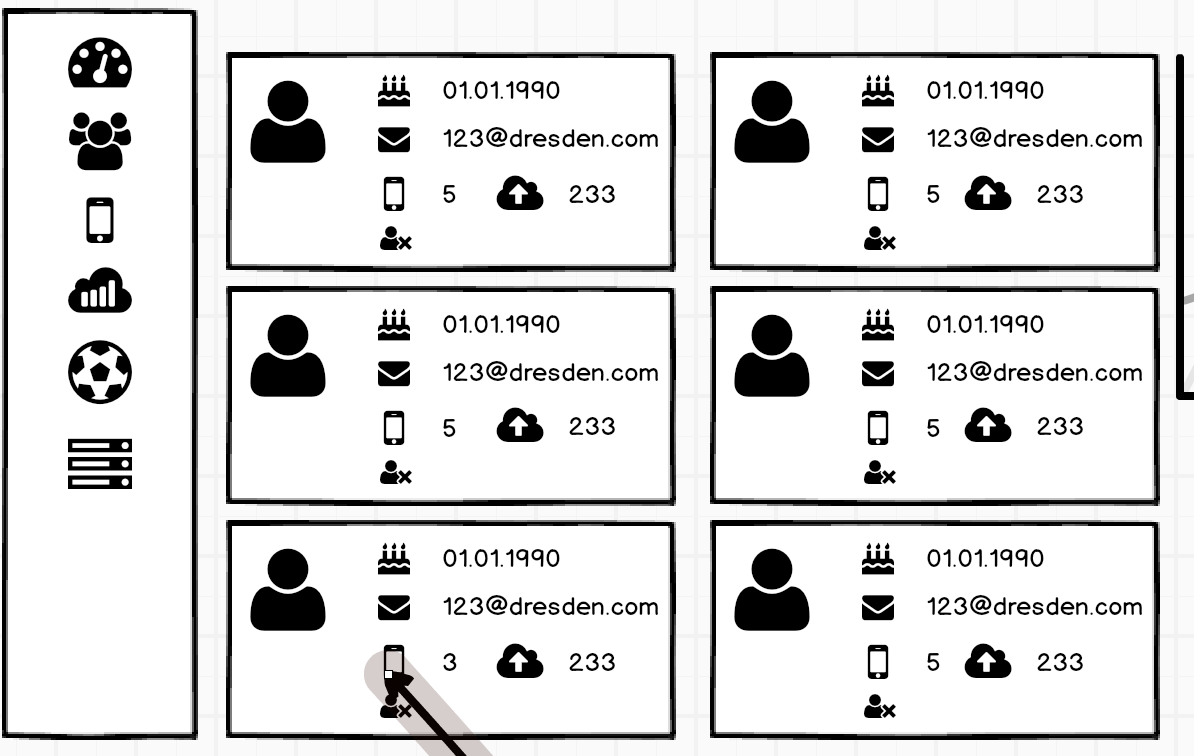
\includegraphics[width=250px, height=120px]{gridview.png}
\caption{Grid View of User}
\label{picture-label16}
\end{figure}\\
In overview module, all statistical data are shown in different chart created by chart.js. In user module, user can be shown with geographical position in Map. In DHT module, tree-style structure has been applied for displaying the neighbors within the K-Bucket of a SANE node.\\\\
A sample of statistical data in overview Moudle.\\
\begin{figure}[htb]
\centering
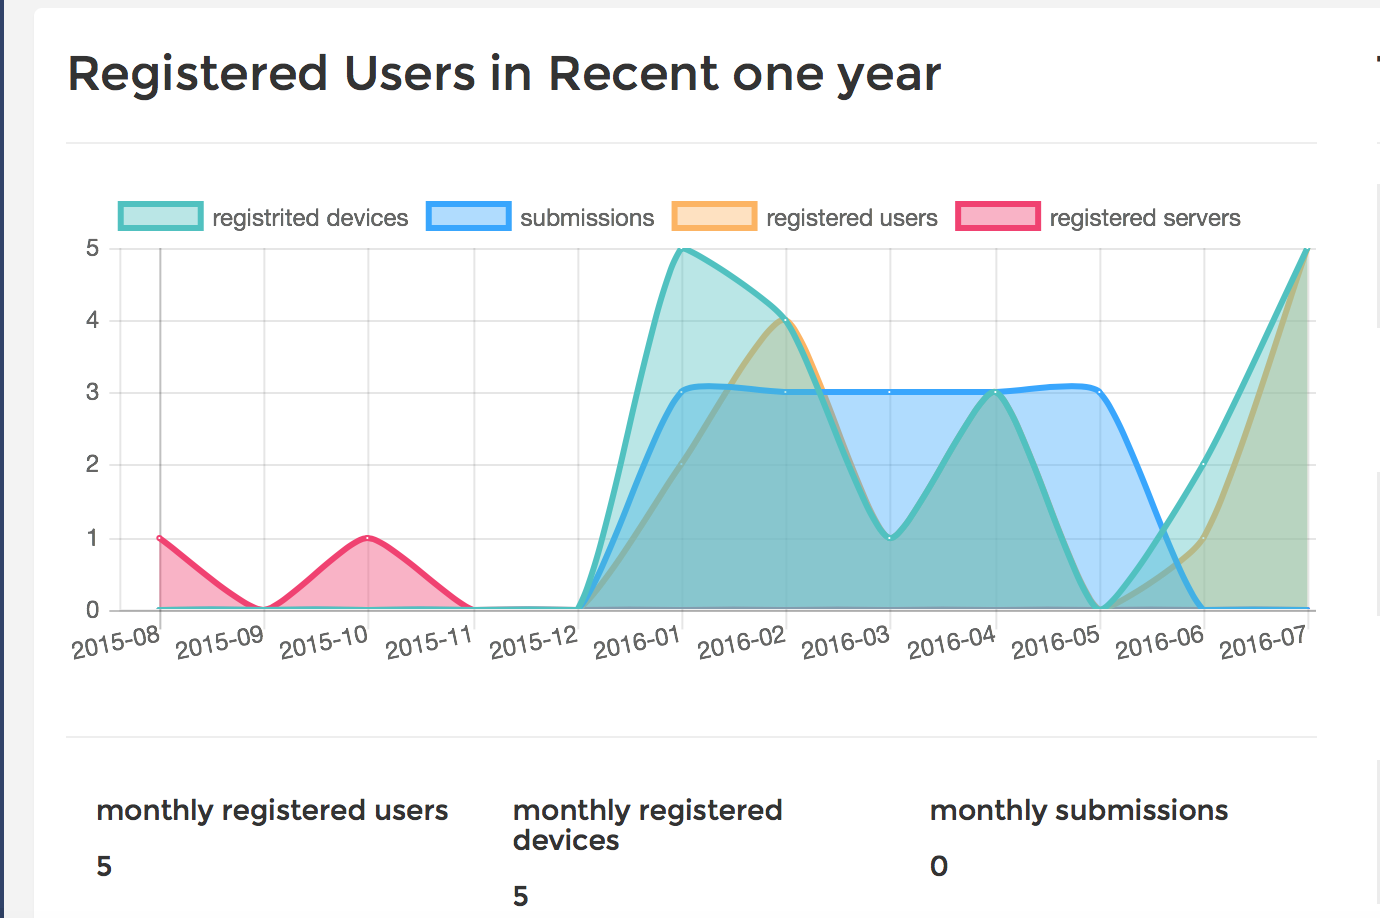
\includegraphics[width=250px, height=120px]{statis.png}
\caption{Statistical View in Overview}
\label{picture-label17}
\end{figure}\\
\subsection{\large Implementation}
The source code of our project is stored privately in Bitbucket. My work was mainly backend implementation. Ji and Chen implemented frontend mainly. Frontend files were compiled as static resources and located in the static folder in backend project.
\subsection{\large Evaluation}
Horizontal Evaluation:
\begin{figure}[htb]
\centering
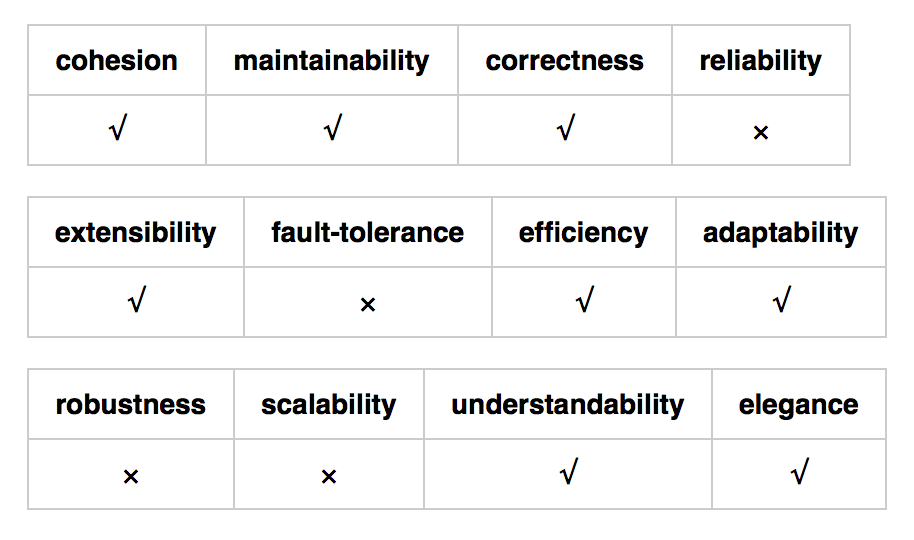
\includegraphics[width=350px, height=150px]{evaluation1.png}
\caption{Horizontal Evaluation}
\label{picture-label18}
\end{figure}\\
From the view of horizontal evaluation, our project meets these criteria:\\\\
Cohesion: Our backend is separated from frontend architecturally. It is easy to maintain, reuse, understand. So it is a system with high cohesion.\\
Maintainability, Extensibility: Besides separation of backend from frontend, backend is based on modular design, frontend is based on AngularJS that has a MVVM (Model-View-ViewModel) pattern. Both sides are easy to maintain and extend.\\
Correctness: Our system performs basically correctly during development and test. It conforms to user’s specific needs and expectations.\\
Efficiency: Our system consumes little resources due to optimized DB operations and basic cache mechanism. The frontend-backend separated architecture has avoided unnecessary data transmission.\\
Adaptability: With zc.buildout and Python itself, our project could be easily deployed on different platforms almost without modification.\\
Understandability: Frontend has different views. The same view has different styles. Statistical data are displayed with different charts. UI components are easy to understand.\\\\
Limitations:\\
Robustness, Reliability, Fault-tolerance: Our system performs well, backend has basic fault-tolerance mechanism. But we have not tested the system for a long period of time under highly concurrent access.\\
Scalability: We have not jet tested scalability of our system in distributed environment.\\
Vertical Evaluation:\\
\begin{figure}[htb]
\centering
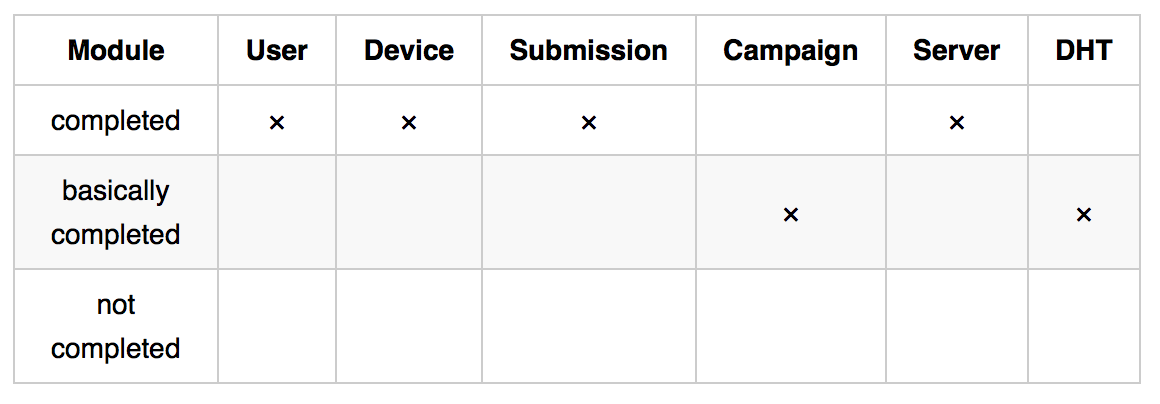
\includegraphics[width=350px, height=150px]{evaluation2.png}
\caption{Vertical Evaluation}
\label{picture-label19}
\end{figure}\\

Modules User, Device, Submission, Server have been completed and met the requirements in concept period. Modules DHT and Campaign have been basically completed. We have only demonstrated how the structure should be displayed. Data was not dynamic generated but static mockup data.
\subsection{\large Summary and Outlook}
This is my first time doing research project. Before this project i have done many other complex practicums. The biggest difference between research project and practicum lies in that i didn't know what to do, what i should do, what i can do at the beginning. Tasks of complex practicums are usually unambiguous, i just need to implement tasks assigned by my tutor.At the beginning of this project i had to analyze the existing project, i had to have meetings with my team members to make sure what were feasible, which module could be completed directly, which module could be completed with the help of some schemas or extensions defined by ourselves, which module was not feasible due to currently ambiguous specifications or other conditions that could not be met as soon as possible. For these currently infeasible tasks, we still had to make compromises to ensure the basic features.\\\\
Since we analyzed the requirements, modeled the system, specified protocols detailedly at the beginning,  we didn't spend too much time on development and modification of protocols or requirements. We have cooperated very well with each other.\\\\
The system has basically met our requirements, the future work, e.g. dynamic DHT data, real mobile device specification, many-to-many users/devices(maybe with modification of DB schema), better display and more features for crowdsourcing servers could be integrated in to existing system without more efforts.

\end{document} % 结束正文